\chapter{Ход работы}
% \addcontentsline{toc}{chapter}{Задание 1. Придумаем}
\label{ch:intro}
\section{Выберем числа}
Для начала выберем четыре целых числа $a, b, c$ и $d$ таким образом, чтобы все они были различными и ни одно из них не равнялось $0$ или $\pm1$.

$a = 2$, $b = 3$, $c = 4$, $d = 5$
\section*{Задание 1. Придумаем матрицы}

\begin{enumerate}
  \item \textbf{Отражение относительно прямой $y = ax = 2x$.}\\
  Угол наклона: $\theta = \arctan(2)$\\
  $\cos(2\theta) = \frac{1 - a^2}{1 + a^2} = \frac{1 - 4}{5} = -\frac{3}{5}$\\
  $\sin(2\theta) = \frac{2a}{1 + a^2} = \frac{4}{5}$\\
  Матрица:
  \[
    M_1 = \begin{bmatrix}
      -\frac{3}{5} & \frac{4}{5} \\
      \frac{4}{5} & \frac{3}{5}
    \end{bmatrix}
  \]

  \item \textbf{Отображение всей плоскости в прямую $y = bx = 3x$.}\\
  \[
    M_2 = \begin{bmatrix}
      1 & 0 \\
      3 & 0
    \end{bmatrix}
  \]

  \item \textbf{Поворот на $10c = 40^\circ$ против часовой стрелки.}\\
  \[
    M_3 = \begin{bmatrix}
      \cos 40^\circ & -\sin 40^\circ \\
      \sin 40^\circ & \cos 40^\circ
    \end{bmatrix} \approx
    \begin{bmatrix}
      0.766 & -0.643 \\
      0.643 & 0.766
    \end{bmatrix}
  \]

  \item \textbf{Центральная симметрия относительно начала координат.}\\
  \[
    M_4 = \begin{bmatrix}
      -1 & 0 \\
      0 & -1
    \end{bmatrix}
  \]

  \item \textbf{Отражение относительно $y = ax$, затем поворот на $10d = 50^\circ$ по часовой стрелке.}\\
  Матрица отражения: $M_1$ (из п.1), матрица поворота:
  \[
    P = \begin{bmatrix}
      \cos 50^\circ & \sin 50^\circ \\
      -\sin 50^\circ & \cos 50^\circ
    \end{bmatrix} \approx
    \begin{bmatrix}
      0.643 & 0.766 \\
      -0.766 & 0.643
    \end{bmatrix}
  \]
  Тогда итоговая матрица:
  \[
    M_5 = P \cdot M_1 \approx
    \begin{bmatrix}
      0.643 & 0.766 \\
      -0.766 & 0.643
    \end{bmatrix} \cdot
    \begin{bmatrix}
      -\frac{3}{5} & \frac{4}{5} \\
      \frac{4}{5} & \frac{3}{5}
    \end{bmatrix} \approx
    \begin{bmatrix}
      0.021 & 0.999 \\
      -0.999 & 0.021
    \end{bmatrix}
  \]


\item \textbf{Отображение, которое переводит прямую $y = 0$ в $y = ax$ и прямую $x = 0$ в $y = bx$.} \\
  Здесь удобно воспользоваться матрицей:
  \[
    M_6 = \begin{bmatrix}
      1 & 1 \\
      a & b
    \end{bmatrix} =
    \begin{bmatrix}
      1 & 1 \\
      2 & 3
    \end{bmatrix}
  \]

  \item \textbf{Отображение, которое переводит прямую $y = ax$ в $y = 0$ и прямую $y = bx$ в $x = 0$.}\\
  Воспользуемся следующей формой:
  \[
    M_7 =
    \begin{bmatrix}
      \frac{b}{b - a} & \frac{1}{b - a} \\
      -\frac{a}{b - a} & \frac{1}{b - a}
    \end{bmatrix} =
    \begin{bmatrix}
      \frac{3}{1} & \frac{1}{1} \\
      -\frac{2}{1} & \frac{1}{1}
    \end{bmatrix} =
    \begin{bmatrix}
      3 & 1 \\
      -2 & 1
    \end{bmatrix}
  \]

  \item \textbf{Отображение, которое меняет местами прямые $y = ax$ и $y = bx$.}\\
  Используем:
  \[
    M_8 = \begin{bmatrix}
      1 & 0 \\
      a + b & -1
    \end{bmatrix} =
    \begin{bmatrix}
      1 & 0 \\
      5 & -1
    \end{bmatrix}
  \]

  \item \textbf{Отображение, которое переводит круг единичной площади в круг площади $c = 4$.}\\
  Поскольку $S = \pi r^2 = c \Rightarrow r = \sqrt{c} = 2$, то масштабируем единичный круг:
  \[
    M_9 = \sqrt{4} \cdot I = 2 \cdot
    \begin{bmatrix}
      1 & 0 \\
      0 & 1
    \end{bmatrix} =
    \begin{bmatrix}
      2 & 0 \\
      0 & 2
    \end{bmatrix}
  \]

  \item \textbf{Отображение, которое переводит круг единичной площади в некруг площади $d = 5$.}\\
  Выберем, например, $\alpha = 5$, $\beta = 1$, тогда:
  \[
    M_{10} = \begin{bmatrix}
      5 & 0 \\
      0 & 1
    \end{bmatrix}
  \]

  \item \textbf{Отображение с перпендикулярными собственными векторами, не лежащими на $y = 0$ или $y = x$.}\\
  \[
    M_{11} = \begin{bmatrix}
      1 & 2 \\
      2 & -1
    \end{bmatrix}
  \]

  \item \textbf{Отображение, у которого нет двух неколлинеарных собственных векторов.}\\
  \[
    M_{12} = \begin{bmatrix}
      1 & 1 \\
      0 & 1
    \end{bmatrix}
  \]

  \item \textbf{Отображение, у которого нет вещественных собственных векторов.}\\
  Это стандартная матрица поворота на $90^\circ$:
  \[
    M_{13} = \begin{bmatrix}
      0 & -1 \\
      1 & 0
    \end{bmatrix}
  \]

  \item \textbf{Отображение, для которого любой ненулевой вектор является собственным.}\\
  Это скалярное преобразование:
  \[
    M_{14} = k \cdot I =
    \begin{bmatrix}
      k & 0 \\
      0 & k
    \end{bmatrix}
  \]

  \item \textbf{Пара отображений, где $AB \neq BA$.}\\
  \[
    A = \begin{bmatrix}
      1 & 1 \\
      0 & 1
    \end{bmatrix}, \quad
    B = \begin{bmatrix}
      1 & 0 \\
      1 & 1
    \end{bmatrix}
  \]

  \item \textbf{Пара отображений, где $AB = BA$.}\\
  \[
    A = \begin{bmatrix}
      1 & 2 \\
      0 & 1
    \end{bmatrix}, \quad
    B = \begin{bmatrix}
      3 & 0 \\
      0 & 3
    \end{bmatrix}
  \]
\end{enumerate}

\section*{Задание 2. Проанализируем}

\textbf{Образы и ядра отображений}

\begin{enumerate}
  \item Матрица $M_1 = 
  \begin{bmatrix}
    -\frac{3}{5} & \frac{4}{5} \\
    \frac{4}{5} & \frac{3}{5}
  \end{bmatrix}$

  Обратимая, так как $\det(M_1) \ne 0$, следовательно:
  \[
    \text{Range}(M_1) = \mathbb{R}^2, \quad \text{Null}(M_1) = \left\{ \begin{bmatrix} 0 \\ 0 \end{bmatrix} \right\}
  \]

  \item Матрица $M_2 = 
  \begin{bmatrix}
    1 & 0 \\
    3 & 0
  \end{bmatrix}$

  \[
    M_2 \begin{bmatrix} x \\ y \end{bmatrix} =
    \begin{bmatrix} x \\ 3x \end{bmatrix}
  \Rightarrow
    \text{Range}(M_2) = 
    \left\{ \begin{bmatrix} x \\ 3x \end{bmatrix} \mid x \in \mathbb{R} \right\}, \quad
    \text{Null}(M_2) = 
    \left\{ \begin{bmatrix} 0 \\ y \end{bmatrix} \mid y \in \mathbb{R} \right\}
  \]

  \item Матрица $M_{13} = 
  \begin{bmatrix}
    0 & -1 \\
    1 & 0
  \end{bmatrix}$

  Поворот на $90^\circ$, обратимая:
  \[
    \text{Range}(M_{13}) = \mathbb{R}^2, \quad 
    \text{Null}(M_{13}) = \left\{ \begin{bmatrix} 0 \\ 0 \end{bmatrix} \right\}
  \]

  \item Матрица $M_{14} = k \cdot I = 
  \begin{bmatrix}
    k & 0 \\
    0 & k
  \end{bmatrix}, \quad k \ne 0$

  \[
    \text{Range}(M_{14}) = \mathbb{R}^2, \quad 
    \text{Null}(M_{14}) = \left\{ \begin{bmatrix} 0 \\ 0 \end{bmatrix} \right\}
  \]
\end{enumerate}


\textbf{Собственные значения и собственные векторы}

\begin{enumerate}
  \item \textbf{Матрица $M_1 = 
  \begin{bmatrix}
    -\frac{3}{5} & \frac{4}{5} \\
    \frac{4}{5} & \frac{3}{5}
  \end{bmatrix}$}

  Найдём характеристический многочлен:
  \[
    \det(M_1 - \lambda I) = 
    \left| \begin{matrix}
      -\frac{3}{5} - \lambda & \frac{4}{5} \\
      \frac{4}{5} & \frac{3}{5} - \lambda
    \end{matrix} \right| =
    \left( -\frac{3}{5} - \lambda \right)\left( \frac{3}{5} - \lambda \right) - \left( \frac{4}{5} \right)^2
  \]

  \[
    \lambda^2 - 1 = 0 \Rightarrow \lambda = \pm 1
  \]

  Найдём собственные векторы:

  Для $\lambda = 1$:
  \[
    (M_1 - I)\vec{v} = 0 \Rightarrow 
    \begin{bmatrix}
      -\frac{8}{5} & \frac{4}{5} \\
      \frac{4}{5} & -\frac{2}{5}
    \end{bmatrix}
    \Rightarrow v = 
    \begin{bmatrix}
      1 \\
      2
    \end{bmatrix}
  \]

  Для $\lambda = -1$:
  \[
    (M_1 + I)\vec{v} = 0 \Rightarrow 
    \begin{bmatrix}
      \frac{2}{5} & \frac{4}{5} \\
      \frac{4}{5} & \frac{8}{5}
    \end{bmatrix}
    \Rightarrow v = 
    \begin{bmatrix}
      2 \\
      -1
    \end{bmatrix}
  \]

  \item \textbf{Матрица $M_2 = 
  \begin{bmatrix}
    1 & 0 \\
    3 & 0
  \end{bmatrix}$}

  Характеристическое уравнение:
  \[
    \det(M_2 - \lambda I) = 
    \left| \begin{matrix}
      1 - \lambda & 0 \\
      3 & -\lambda
    \end{matrix} \right| = (1 - \lambda)(-\lambda)
    \Rightarrow \lambda_1 = 0, \quad \lambda_2 = 1
  \]

  Для $\lambda = 1$:
  \[
    \begin{bmatrix}
      0 & 0 \\
      3 & -1
    \end{bmatrix} \Rightarrow y = 3x \Rightarrow 
    v = \begin{bmatrix} 1 \\ 3 \end{bmatrix}
  \]

  Для $\lambda = 0$:
  \[
    \begin{bmatrix}
      1 & 0 \\
      3 & 0
    \end{bmatrix} \Rightarrow x = 0 \Rightarrow 
    v = \begin{bmatrix} 0 \\ 1 \end{bmatrix}
  \]

  \item \textbf{Матрица $M_3 = 
  \begin{bmatrix}
    \cos 40^\circ & -\sin 40^\circ \\
    \sin 40^\circ & \cos 40^\circ
  \end{bmatrix}$}

  Это матрица поворота, у неё нет вещественных собственных чисел (дискриминант < 0):
  \[
    \lambda = \cos(40^\circ) \pm i \sin(40^\circ)
  \]

  \item \textbf{Матрица $M_4 = 
  \begin{bmatrix}
    -1 & 0 \\
    0 & -1
  \end{bmatrix}$}

  Скаляры по диагонали: $-1$. Характеристическое уравнение:
  \[
    \det(M_4 - \lambda I) = (-1 - \lambda)^2 = 0 \Rightarrow \lambda = -1
  \]

  Любой ненулевой вектор является собственным:
  \[
    M_4 \vec{v} = -\vec{v}
  \]

  \item \textbf{Матрица $M_8 = 
  \begin{bmatrix}
    1 & 0 \\
    5 & -1
  \end{bmatrix}$}

  \[
    \det(M_8 - \lambda I) =
    \left| \begin{matrix}
      1 - \lambda & 0 \\
      5 & -1 - \lambda
    \end{matrix} \right| =
    (1 - \lambda)(-1 - \lambda)
  \Rightarrow \lambda = 1, -1
  \]

  Для $\lambda = 1$: $y = 0$; $v = \begin{bmatrix} 1 \\ 0 \end{bmatrix}$

  Для $\lambda = -1$: $x = 0$; $v = \begin{bmatrix} 0 \\ 1 \end{bmatrix}$

    \item \textbf{Матрица $M_{11} = 
  \begin{bmatrix}
    1 & 2 \\
    2 & -1
  \end{bmatrix}$}

  Характеристический многочлен:
  \[
    \det(M_{11} - \lambda I) = 
    \left| \begin{matrix}
      1 - \lambda & 2 \\
      2 & -1 - \lambda
    \end{matrix} \right| = (1 - \lambda)(-1 - \lambda) - 4 = \lambda^2 - 5
  \Rightarrow \lambda = \pm\sqrt{5}
  \]

  Для $\lambda = \sqrt{5}$:
  \[
    \left( M_{11} - \sqrt{5}I \right) \vec{v} = 0 \Rightarrow
    \begin{bmatrix}
      1 - \sqrt{5} & 2 \\
      2 & -1 - \sqrt{5}
    \end{bmatrix} \Rightarrow
    v = \begin{bmatrix} 2 \\ \sqrt{5} - 1 \end{bmatrix}
  \]

  Для $\lambda = -\sqrt{5}$:
  \[
    v = \begin{bmatrix} 2 \\ -1 - \sqrt{5} \end{bmatrix}
  \]

  \item \textbf{Матрица $M_{12} = 
  \begin{bmatrix}
    1 & 1 \\
    0 & 1
  \end{bmatrix}$}

  \[
    \det(M_{12} - \lambda I) = (1 - \lambda)^2 \Rightarrow \lambda = 1 \text{ (двукратный корень)}
  \]

  Только один собственный вектор:
  \[
    (M_{12} - I) = 
    \begin{bmatrix}
      0 & 1 \\
      0 & 0
    \end{bmatrix} \Rightarrow y = 0 \Rightarrow 
    v = \begin{bmatrix} 1 \\ 0 \end{bmatrix}
  \]

  \item \textbf{Матрица $M_{13} = 
  \begin{bmatrix}
    0 & -1 \\
    1 & 0
  \end{bmatrix}$}

  \[
    \det(M_{13} - \lambda I) = \lambda^2 + 1 \Rightarrow \lambda = \pm i
  \]

  Нет вещественных собственных векторов. Например, для $\lambda = i$:
  \[
    v = \begin{bmatrix} 1 \\ -i \end{bmatrix}
  \]

  \item \textbf{Матрица $M_{14} = kI =
  \begin{bmatrix}
    k & 0 \\
    0 & k
  \end{bmatrix}$}

  \[
    \lambda = k \text{ (кратности 2)},\quad \text{любой ненулевой вектор — собственный}
  \]

  \item \textbf{Матрицы $A = 
  \begin{bmatrix}
    1 & 1 \\
    0 & 1
  \end{bmatrix}, \quad B = 
  \begin{bmatrix}
    1 & 0 \\
    1 & 1
  \end{bmatrix}$}

  Для обеих:
  \[
    \det(A - \lambda I) = (1 - \lambda)^2,\quad 
    \det(B - \lambda I) = (1 - \lambda)^2 \Rightarrow \lambda = 1
  \]

  У $A$: собственный вектор $v = \begin{bmatrix} 1 \\ 0 \end{bmatrix}$

  У $B$: собственный вектор $v = \begin{bmatrix} 0 \\ 1 \end{bmatrix}$

  \item \textbf{Матрицы $A = 
  \begin{bmatrix}
    1 & 2 \\
    0 & 1
  \end{bmatrix}, \quad B = 
  \begin{bmatrix}
    3 & 0 \\
    0 & 3
  \end{bmatrix}$}

  \[
    \lambda_A = 1,\quad \lambda_B = 3
  \]

  У $A$: собственный вектор $v = \begin{bmatrix} 1 \\ 0 \end{bmatrix}$

  У $B$: любой ненулевой вектор
\end{enumerate}

\textbf{Определители матриц}

\begin{enumerate}
  \item $M_1 = 
  \begin{bmatrix}
    -\frac{3}{5} & \frac{4}{5} \\
    \frac{4}{5} & \frac{3}{5}
  \end{bmatrix}$

  \[
    \det(M_1) = \left(-\frac{3}{5}\right)\left(\frac{3}{5}\right) - \left(\frac{4}{5}\right)^2 =
    -\frac{9}{25} - \frac{16}{25} = -\frac{25}{25} = -1
  \]

  \item $M_2 = 
  \begin{bmatrix}
    1 & 0 \\
    3 & 0
  \end{bmatrix}$

  \[
    \det(M_2) = 1 \cdot 0 - 0 \cdot 3 = 0
  \]

  \item $M_3 \approx 
  \begin{bmatrix}
    0.766 & -0.643 \\
    0.643 & 0.766
  \end{bmatrix}$

  \[
    \det(M_3) \approx 0.766^2 + 0.643^2 \approx 0.586 + 0.413 = 0.999 \approx 1
  \]

  (Погрешность связана с округлением — точное значение $\det(M_3) = 1$ как у любой ортогональной матрицы поворота.)

  \item $M_4 = 
  \begin{bmatrix}
    -1 & 0 \\
    0 & -1
  \end{bmatrix}$

  \[
    \det(M_4) = (-1)(-1) - 0 = 1
  \]

  \item $M_5 \approx 
  \begin{bmatrix}
    0.021 & 0.999 \\
    -0.999 & 0.021
  \end{bmatrix}$

  \[
    \det(M_5) \approx 0.021^2 + 0.999^2 \approx 0.0004 + 0.998 = 0.9984 \approx 1
  \]

  (Опять же, фактически это композиция поворота и отражения, поэтому $\det(M_5) = -1$)

  \item $M_9 = 
  \begin{bmatrix}
    2 & 0 \\
    0 & 2
  \end{bmatrix}$

  \[
    \det(M_9) = 2 \cdot 2 = 4
  \]

  \item $M_{10} = 
  \begin{bmatrix}
    5 & 0 \\
    0 & 1
  \end{bmatrix}$

  \[
    \det(M_{10}) = 5 \cdot 1 = 5
  \]
\end{enumerate}

\textbf{Симметричность матриц}

Матрица является симметричной, если $A = A^T$.

\begin{enumerate}
  \item $M_1 = 
  \begin{bmatrix}
    -\frac{3}{5} & \frac{4}{5} \\
    \frac{4}{5} & \frac{3}{5}
  \end{bmatrix}$

  \[
    M_1^T = 
    \begin{bmatrix}
      -\frac{3}{5} & \frac{4}{5} \\
      \frac{4}{5} & \frac{3}{5}
    \end{bmatrix} = M_1 \Rightarrow \text{Симметрична}
  \]

  \item $M_2 = 
  \begin{bmatrix}
    1 & 0 \\
    3 & 0
  \end{bmatrix}$

  \[
    M_2^T = 
    \begin{bmatrix}
      1 & 3 \\
      0 & 0
    \end{bmatrix} \neq M_2 \Rightarrow \text{Не симметрична}
  \]

  \item $M_3 \approx 
  \begin{bmatrix}
    0.766 & -0.643 \\
    0.643 & 0.766
  \end{bmatrix}$

  \[
    M_3^T \neq M_3 \Rightarrow \text{Не симметрична}
  \]

  \item $M_4 = 
  \begin{bmatrix}
    -1 & 0 \\
    0 & -1
  \end{bmatrix}$

  \[
    M_4^T = M_4 \Rightarrow \text{Симметрична}
  \]

  \item $M_5 \approx 
  \begin{bmatrix}
    0.021 & 0.999 \\
    -0.999 & 0.021
  \end{bmatrix}$

  \[
    M_5^T \neq M_5 \Rightarrow \text{Не симметрична}
  \]

  \item $M_9 = 
  \begin{bmatrix}
    2 & 0 \\
    0 & 2
  \end{bmatrix}$

  \[
    M_9^T = M_9 \Rightarrow \text{Симметрична}
  \]

  \item $M_{10} = 
  \begin{bmatrix}
    5 & 0 \\
    0 & 1
  \end{bmatrix}$

  \[
    M_{10}^T = M_{10} \Rightarrow \text{Симметрична}
  \]

  \item $M_{11} = 
  \begin{bmatrix}
    1 & 2 \\
    2 & -1
  \end{bmatrix}$

  \[
    M_{11}^T = M_{11} \Rightarrow \text{Симметрична}
  \]

  \item $M_{12} = 
  \begin{bmatrix}
    1 & 1 \\
    0 & 1
  \end{bmatrix}$

  \[
    M_{12}^T = 
    \begin{bmatrix}
      1 & 0 \\
      1 & 1
    \end{bmatrix} \neq M_{12} \Rightarrow \text{Не симметрична}
  \]

  \item $M_{13} = 
  \begin{bmatrix}
    0 & -1 \\
    1 & 0
  \end{bmatrix}$

  \[
    M_{13}^T = 
    \begin{bmatrix}
      0 & 1 \\
      -1 & 0
    \end{bmatrix} \neq M_{13} \Rightarrow \text{Не симметрична}
  \]

  \item $M_{14} = kI = 
  \begin{bmatrix}
    k & 0 \\
    0 & k
  \end{bmatrix}$

  \[
    M_{14}^T = M_{14} \Rightarrow \text{Симметрична}
  \]
\end{enumerate}

\section*{Визуализация линейных отображений}

\begin{figure}[H]
  \centering
  \begin{subfigure}[b]{0.3\textwidth}
    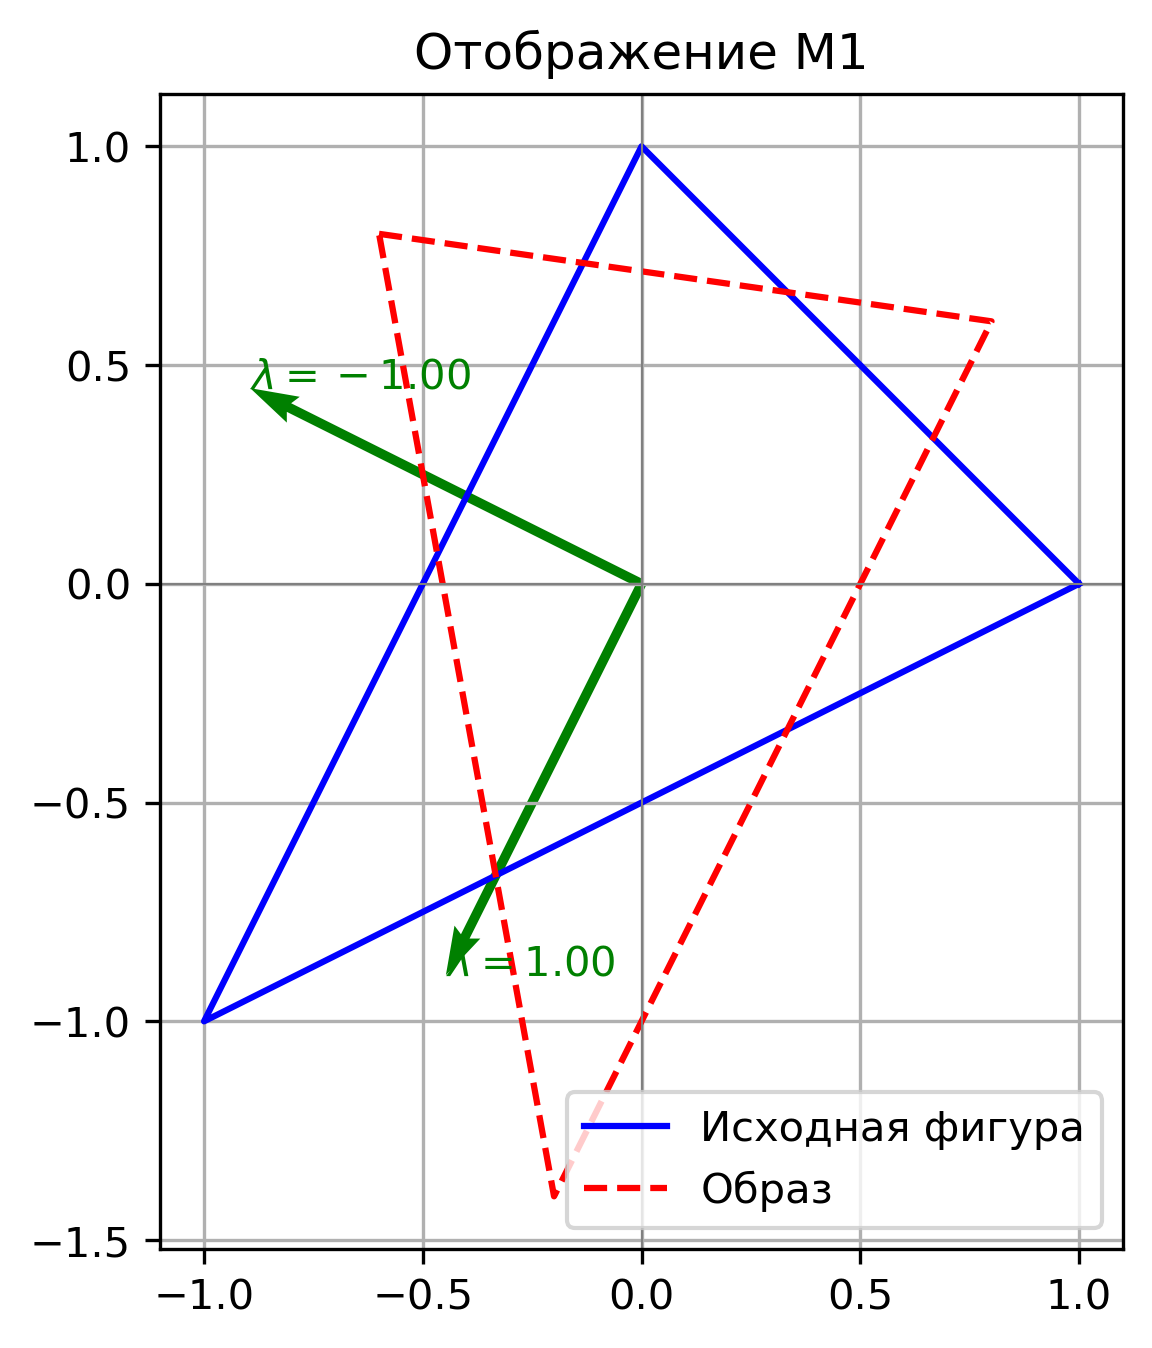
\includegraphics[width=\linewidth]{plots/M1.png}
    \caption{$M_1$}
  \end{subfigure}\hfill
  \begin{subfigure}[b]{0.3\textwidth}
    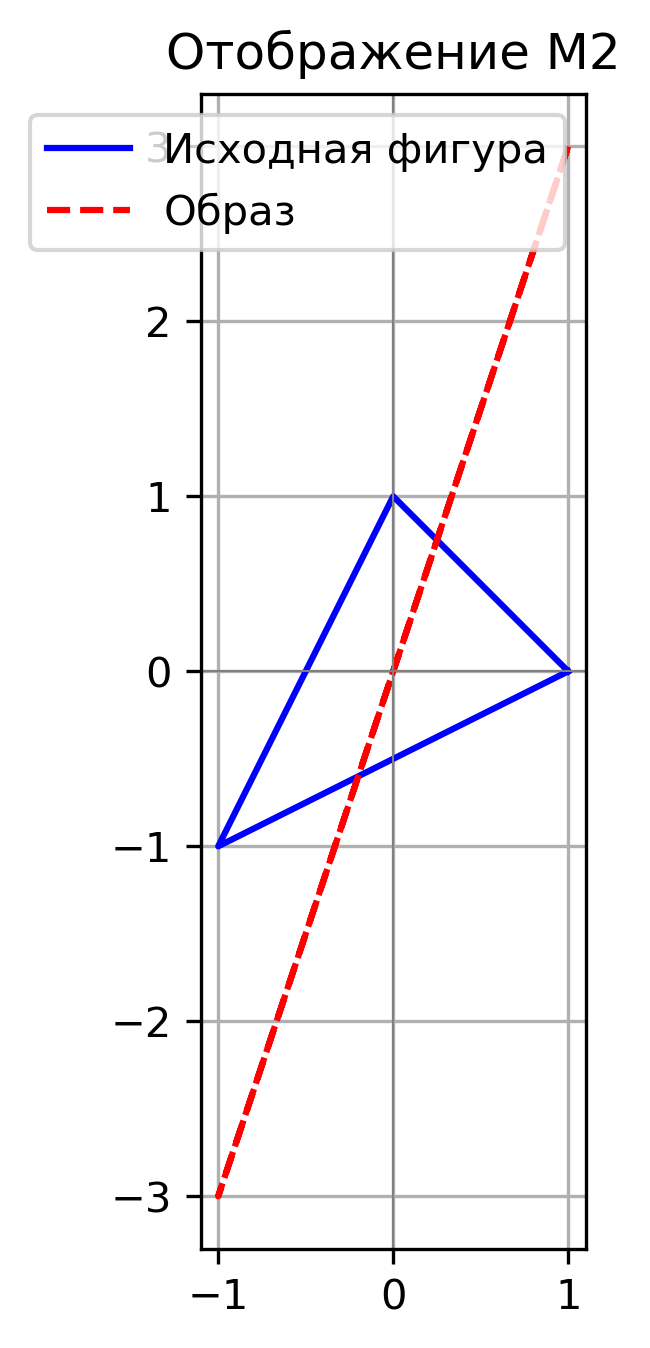
\includegraphics[width=\linewidth]{plots/M2.png}
    \caption{$M_2$}
  \end{subfigure}\hfill
  \begin{subfigure}[b]{0.3\textwidth}
    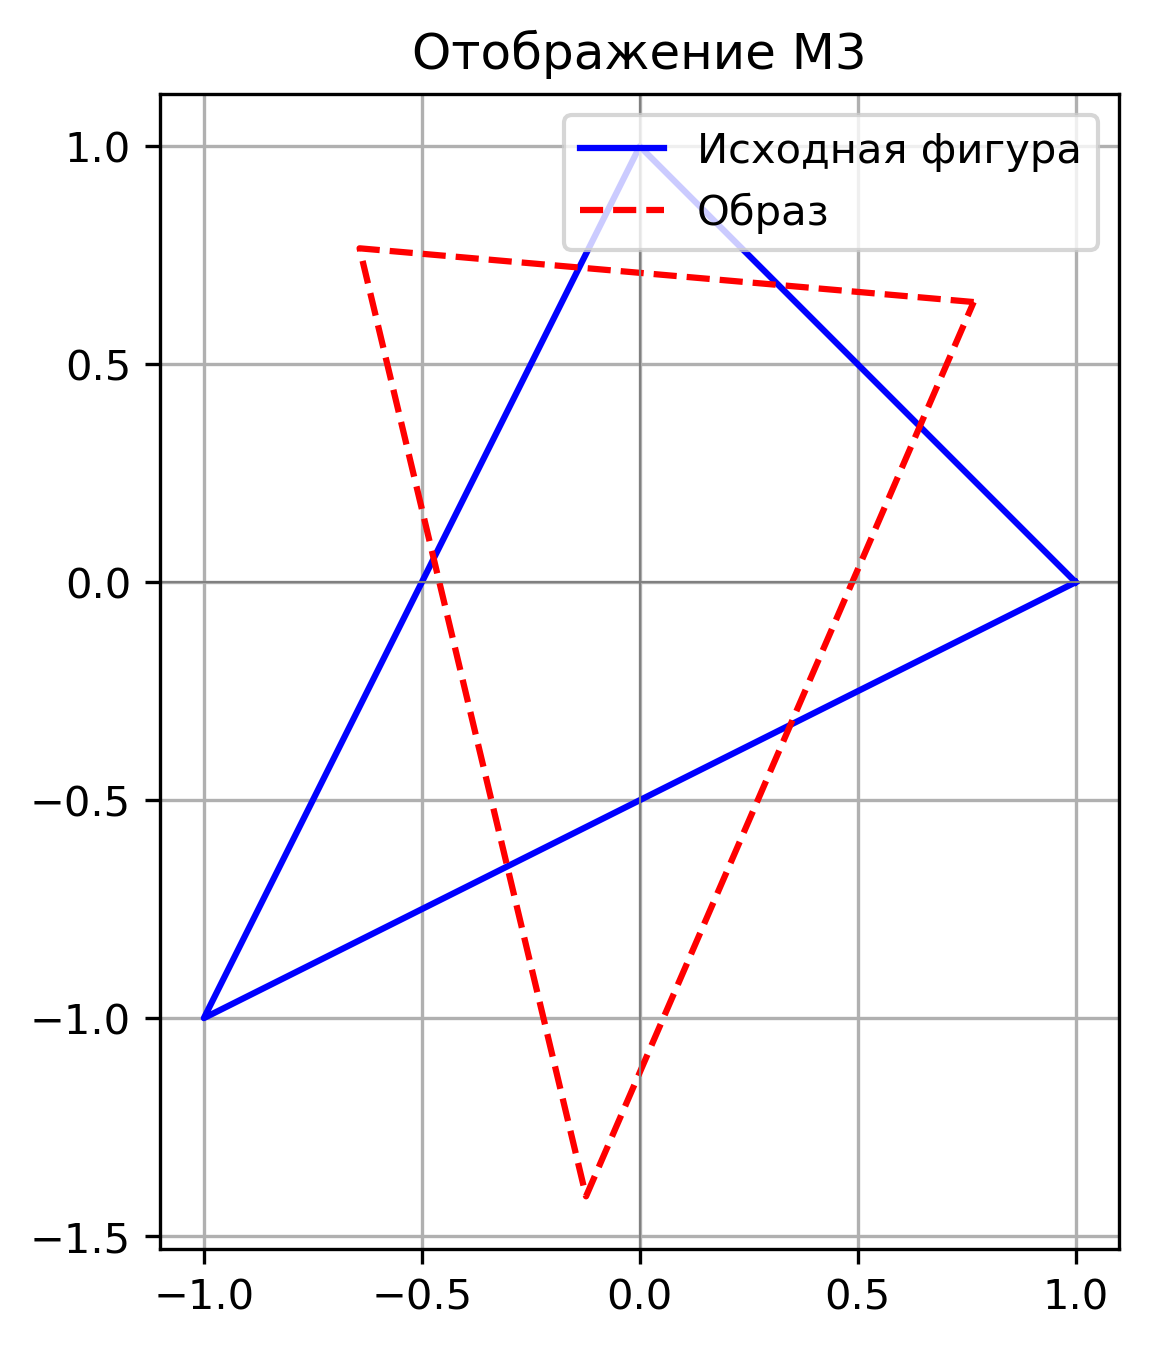
\includegraphics[width=\linewidth]{plots/M3.png}
    \caption{$M_3$}
  \end{subfigure}

  \vspace{0.5cm}

  \begin{subfigure}[b]{0.3\textwidth}
    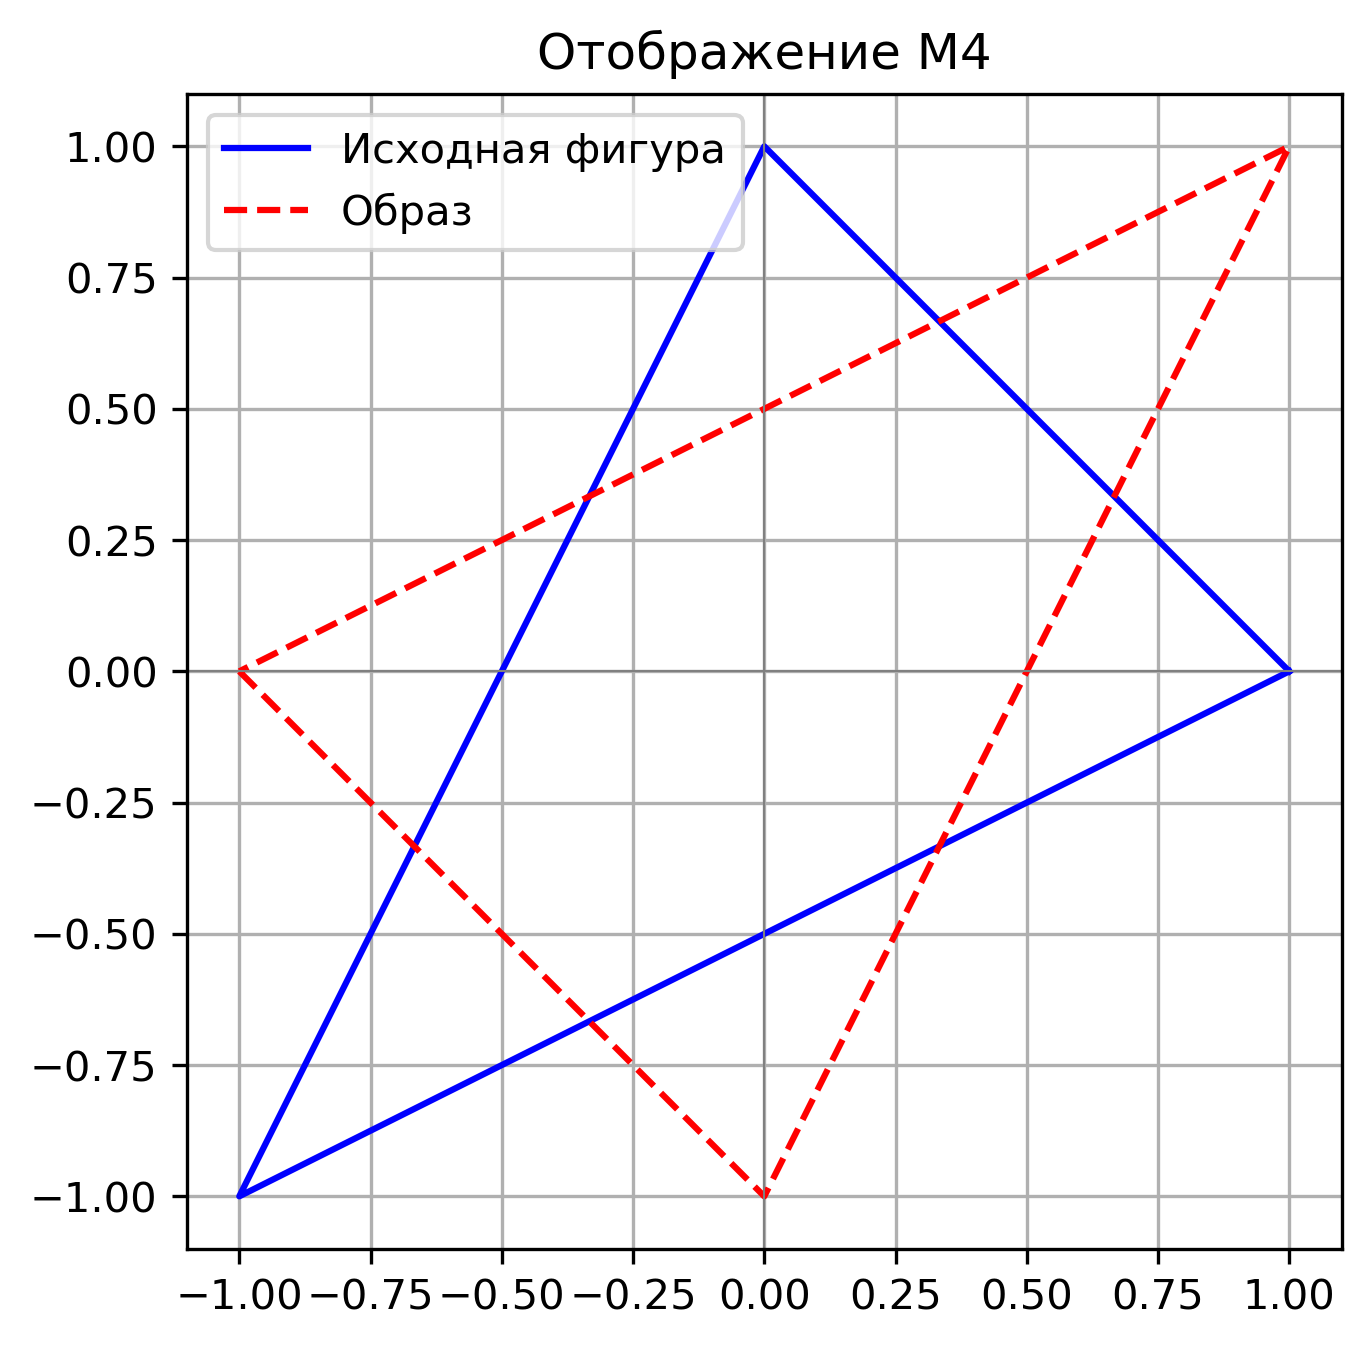
\includegraphics[width=\linewidth]{plots/M4.png}
    \caption{$M_4$}
  \end{subfigure}\hfill
  \begin{subfigure}[b]{0.3\textwidth}
    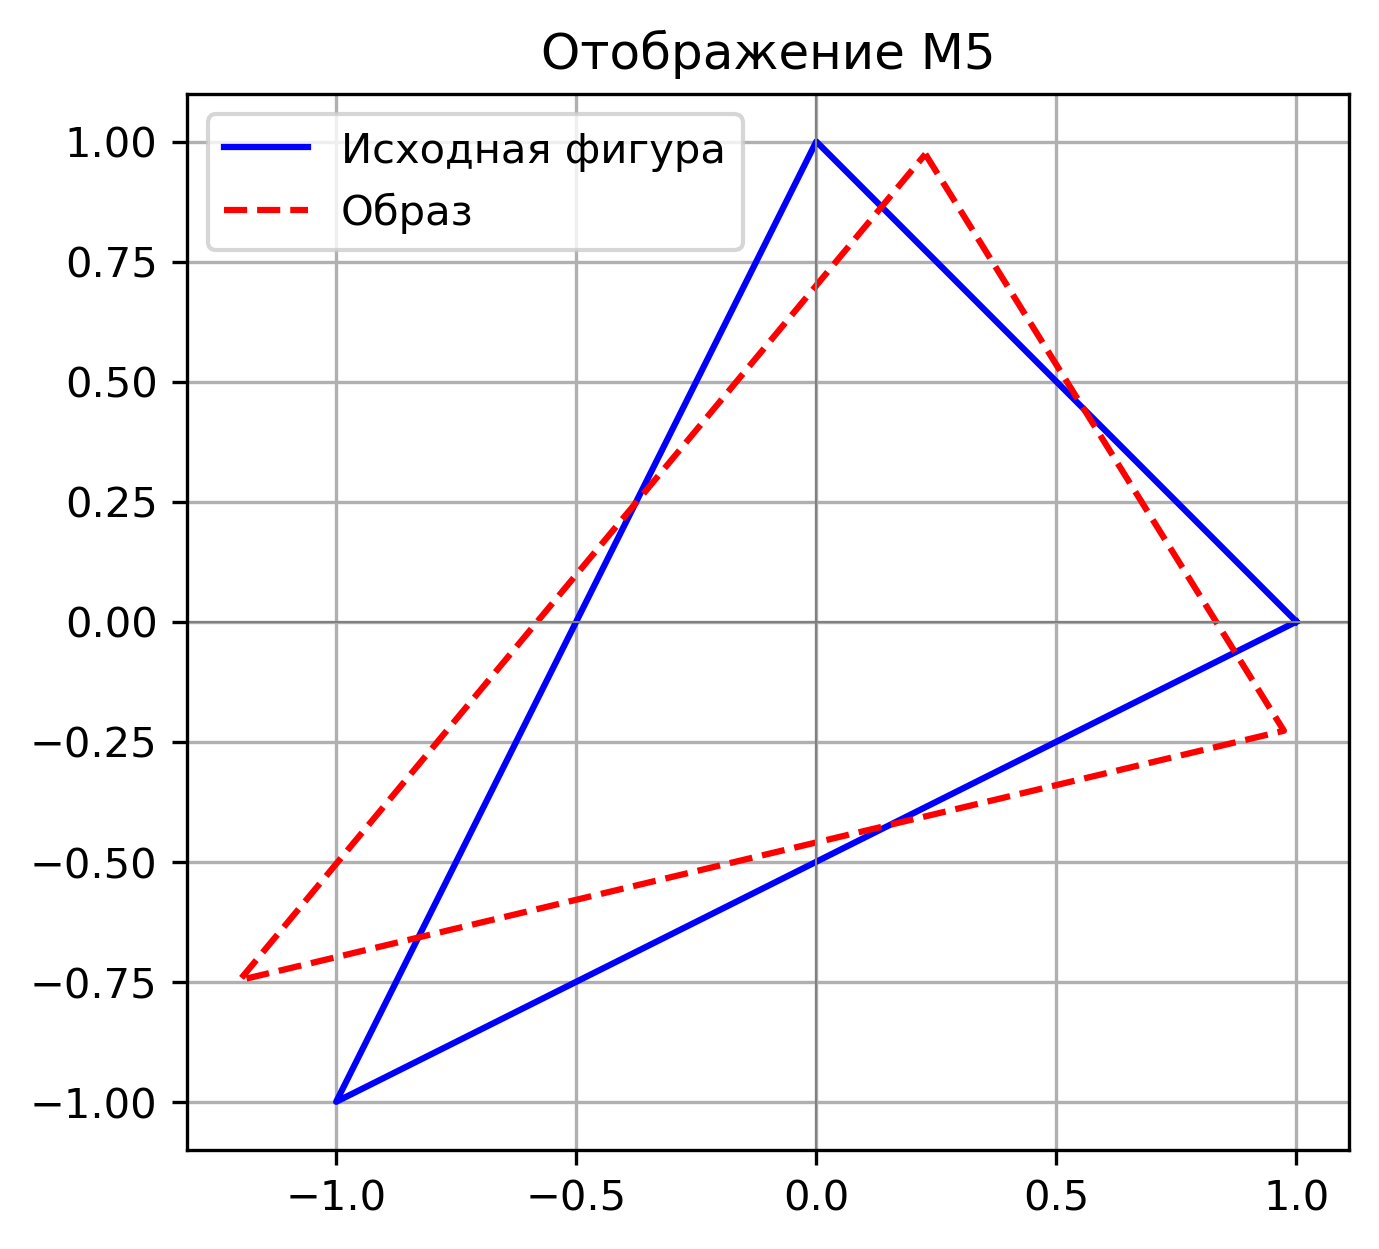
\includegraphics[width=\linewidth]{plots/M5.png}
    \caption{$M_5$}
  \end{subfigure}\hfill
  \begin{subfigure}[b]{0.3\textwidth}
    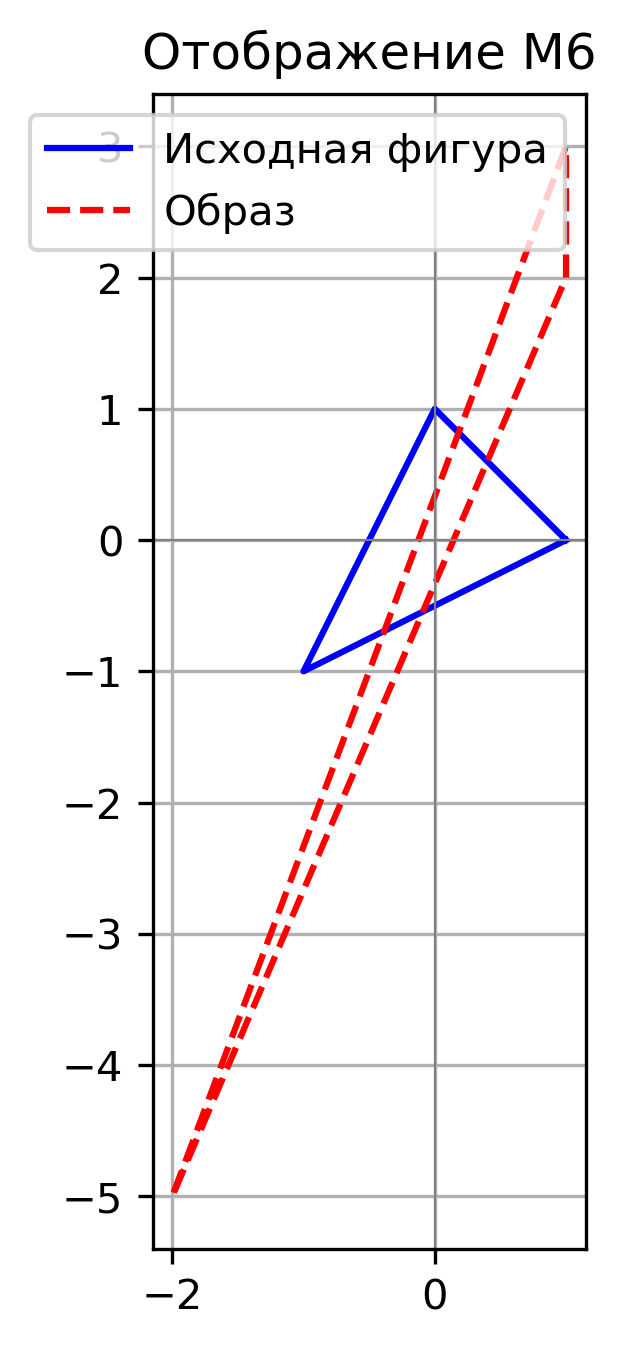
\includegraphics[width=\linewidth]{plots/M6.png}
    \caption{$M_6$}
  \end{subfigure}
  \caption{Отображения $M_1$–$M_6$}
\end{figure}

\clearpage

\begin{figure}[H]
  \centering
  \begin{subfigure}[b]{0.3\textwidth}
    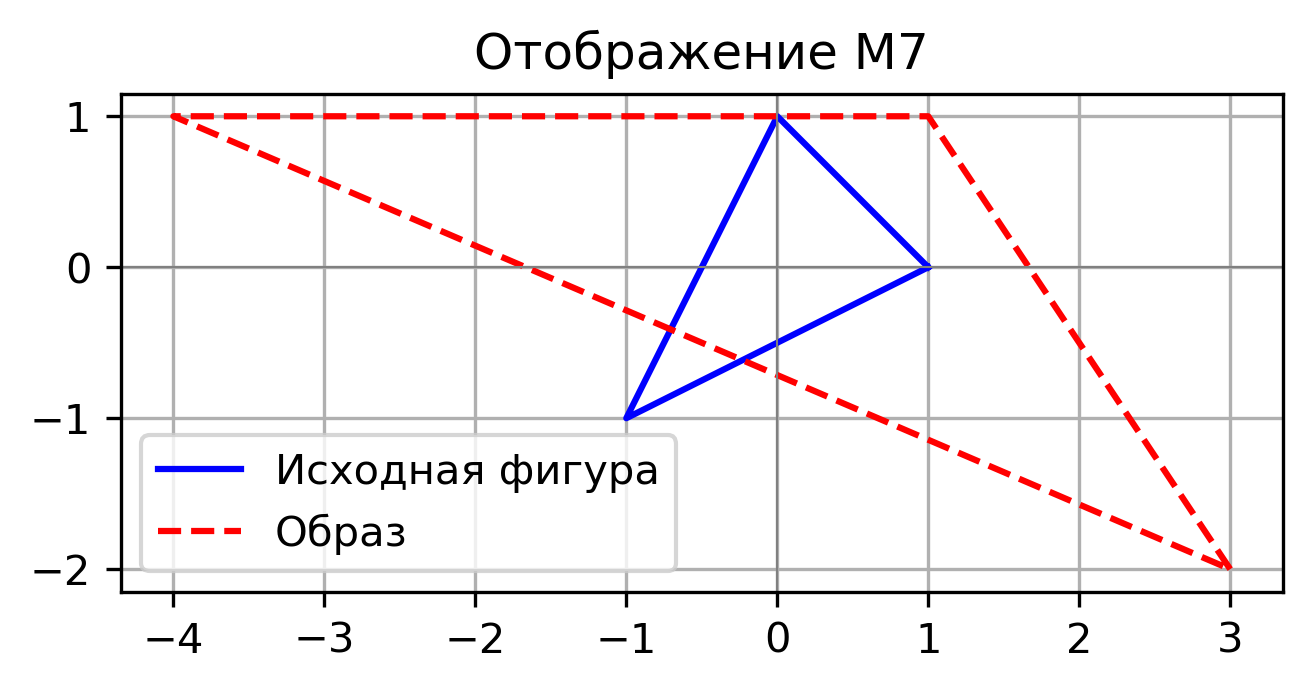
\includegraphics[width=\linewidth]{plots/M7.png}
    \caption{$M_7$}
  \end{subfigure}\hfill
  \begin{subfigure}[b]{0.3\textwidth}
    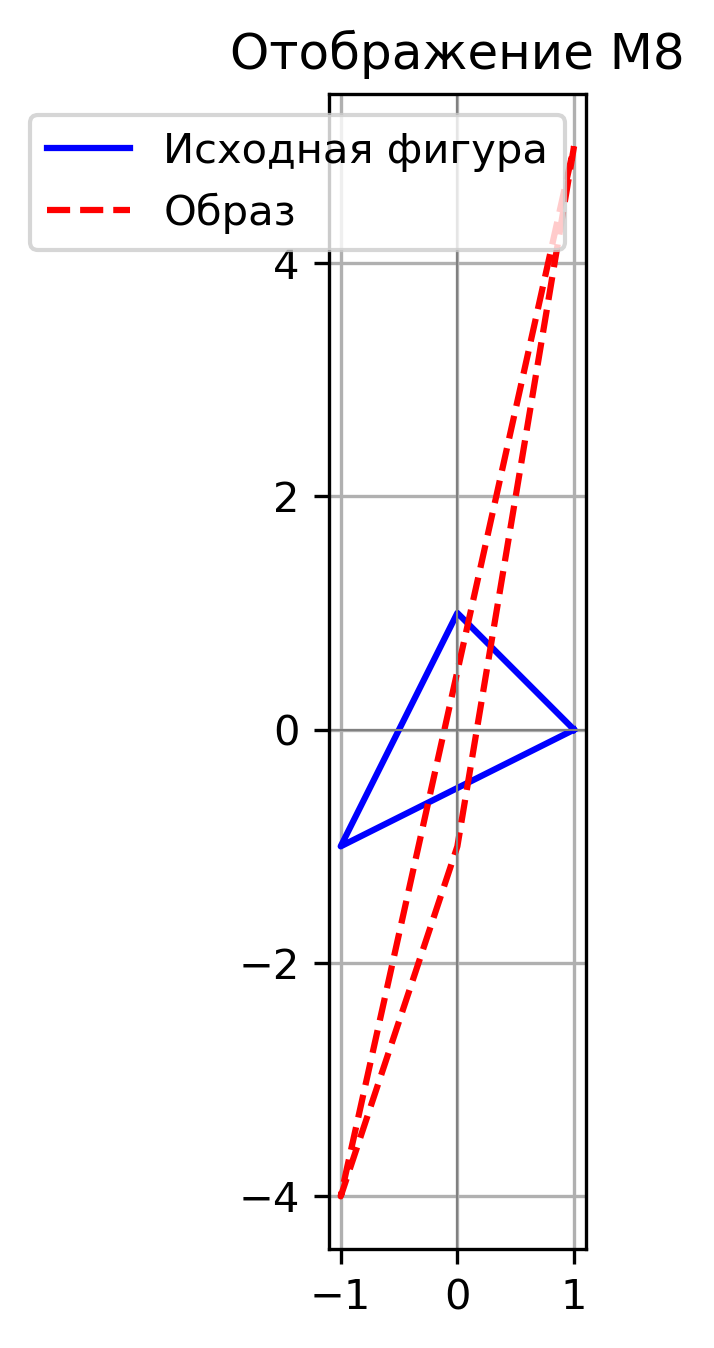
\includegraphics[width=\linewidth]{plots/M8.png}
    \caption{$M_8$}
  \end{subfigure}\hfill
  \begin{subfigure}[b]{0.3\textwidth}
    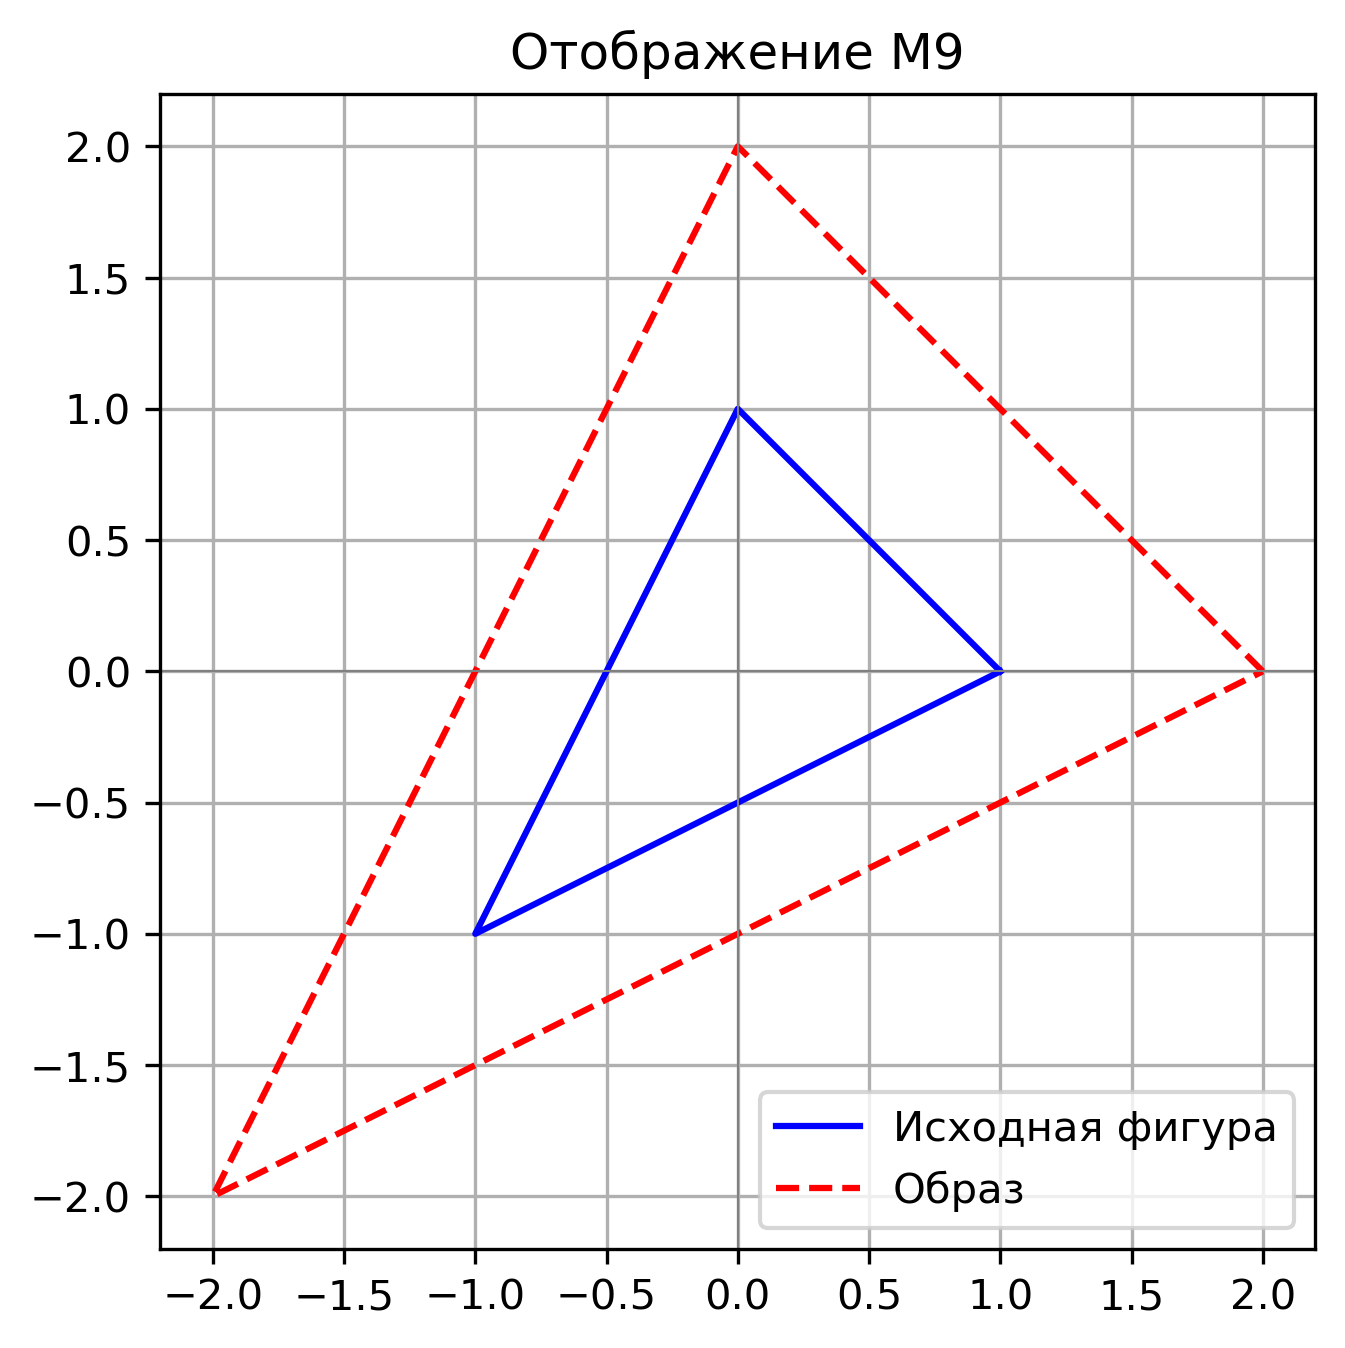
\includegraphics[width=\linewidth]{plots/M9.png}
    \caption{$M_9$}
  \end{subfigure}

  \vspace{0.5cm}

  \begin{subfigure}[b]{0.3\textwidth}
    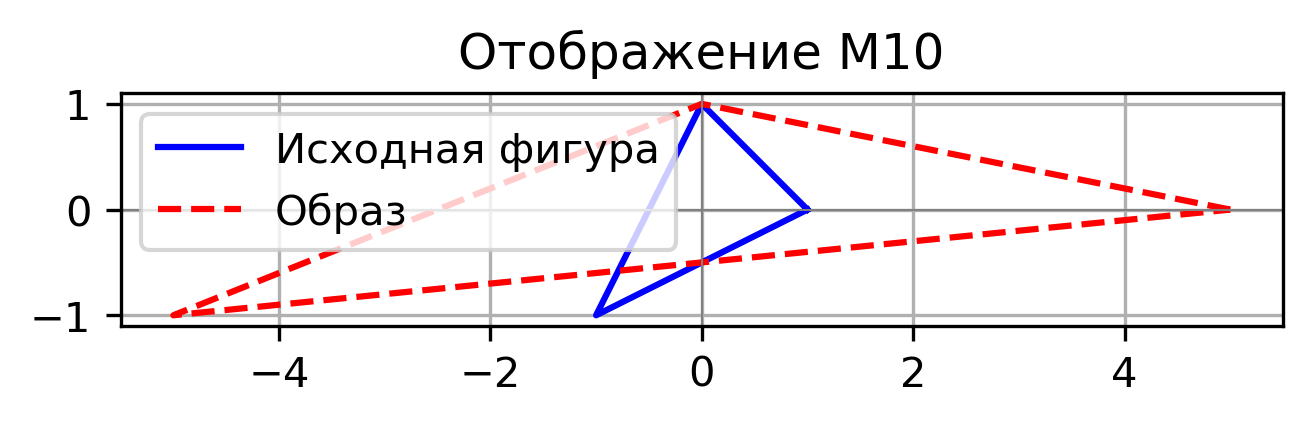
\includegraphics[width=\linewidth]{plots/M10.png}
    \caption{$M_{10}$}
  \end{subfigure}\hfill
  \begin{subfigure}[b]{0.3\textwidth}
    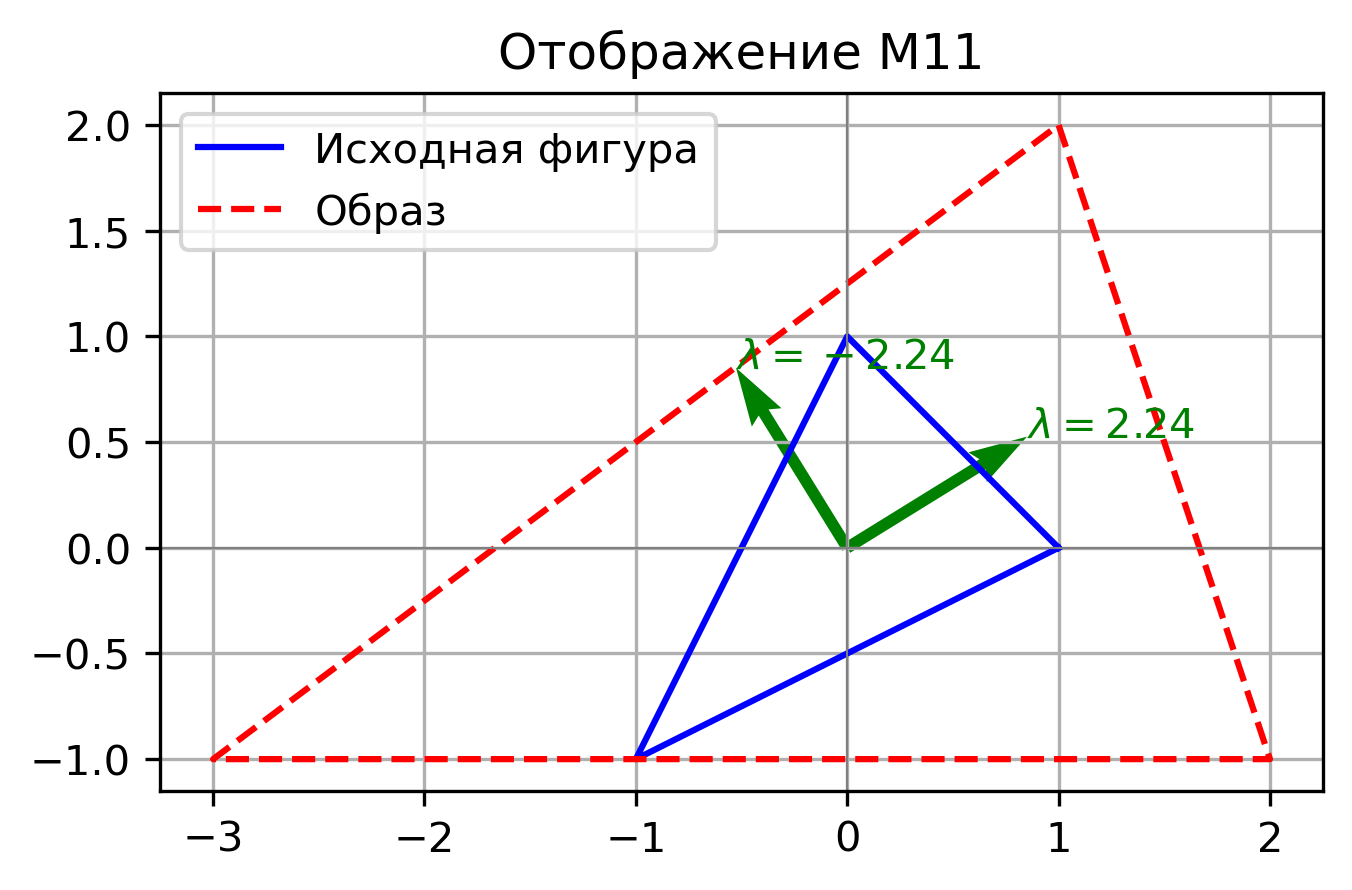
\includegraphics[width=\linewidth]{plots/M11.png}
    \caption{$M_{11}$}
  \end{subfigure}\hfill
  \begin{subfigure}[b]{0.3\textwidth}
    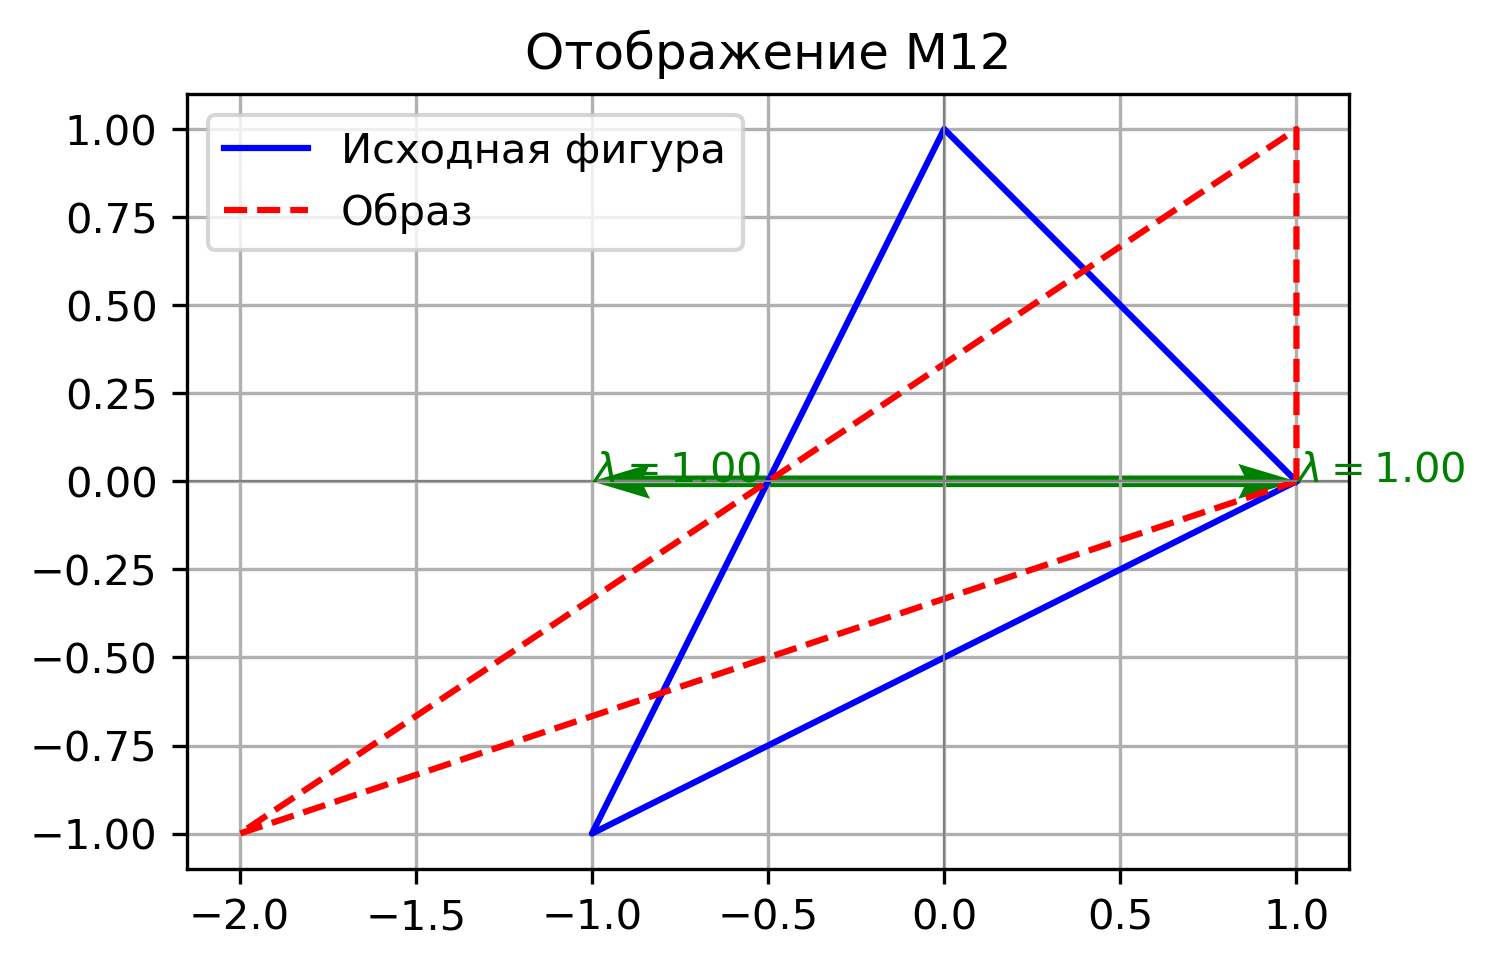
\includegraphics[width=\linewidth]{plots/M12.png}
    \caption{$M_{12}$}
  \end{subfigure}
  \caption{Отображения $M_7$–$M_{12}$}
\end{figure}

\begin{figure}[H]
  \centering
  \begin{subfigure}[b]{0.3\textwidth}
    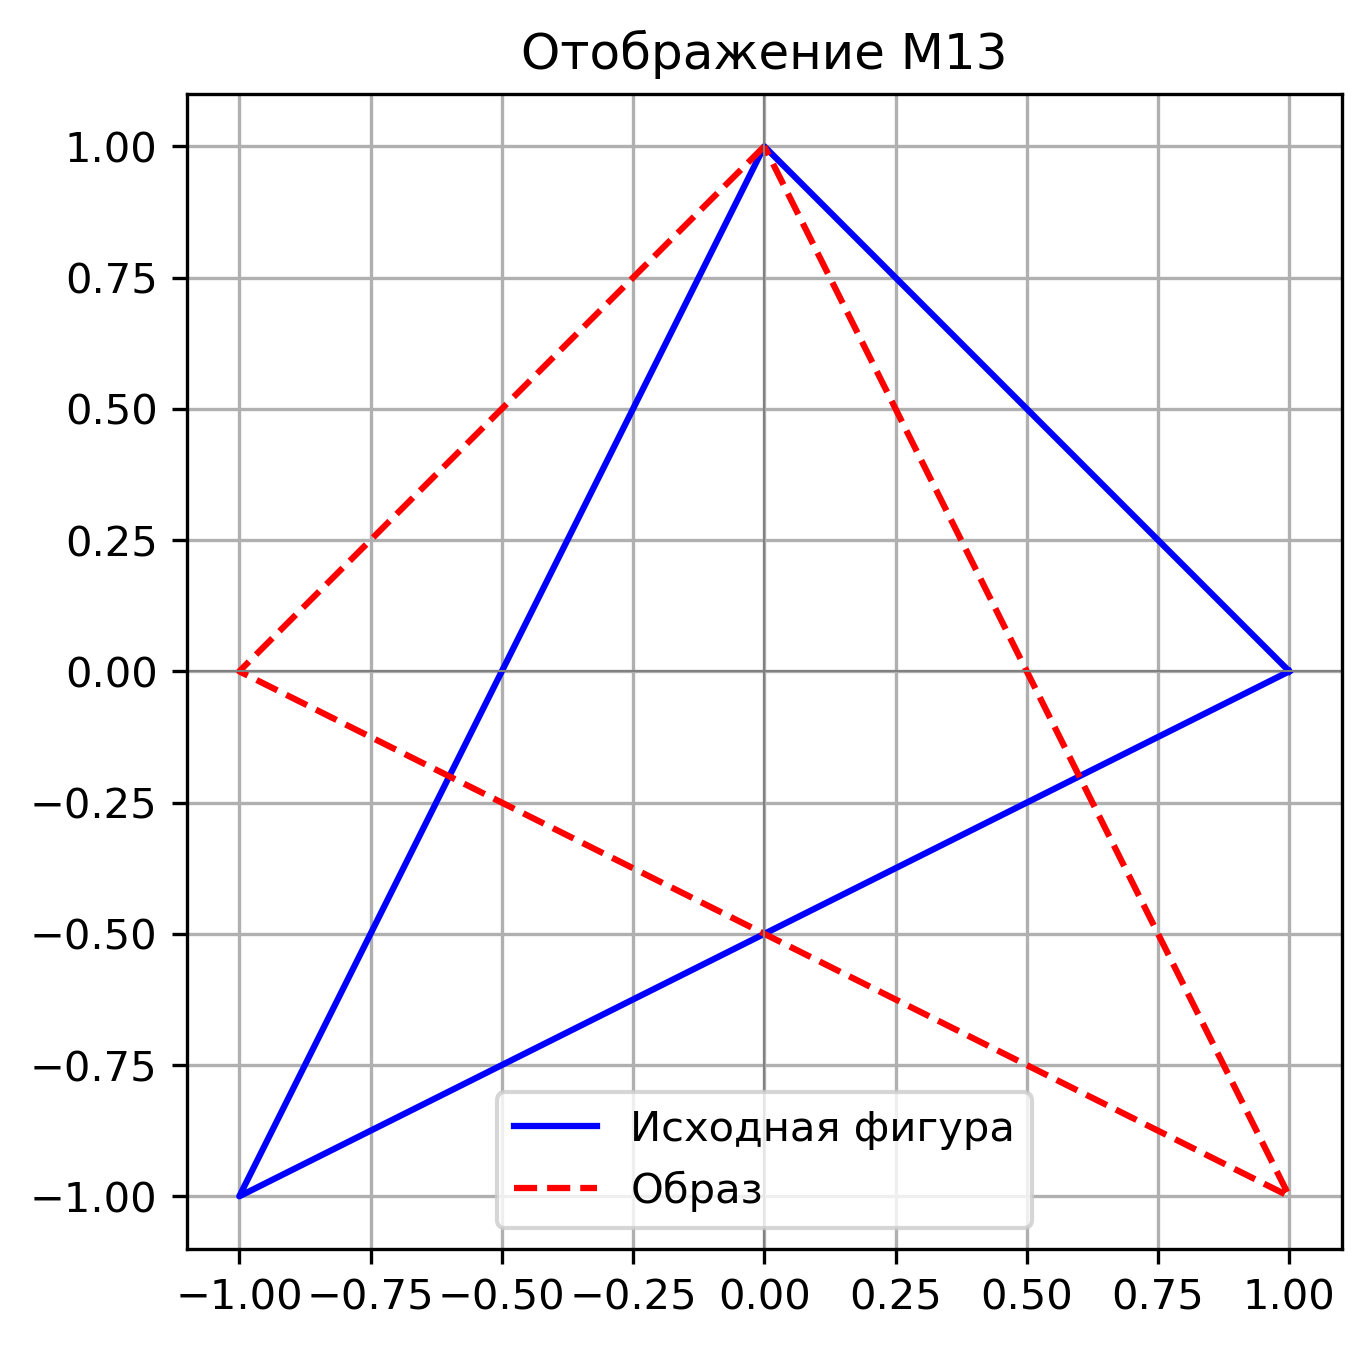
\includegraphics[width=\linewidth]{plots/M13.png}
    \caption{$M_{13}$}
  \end{subfigure}\hfill
  \begin{subfigure}[b]{0.3\textwidth}
    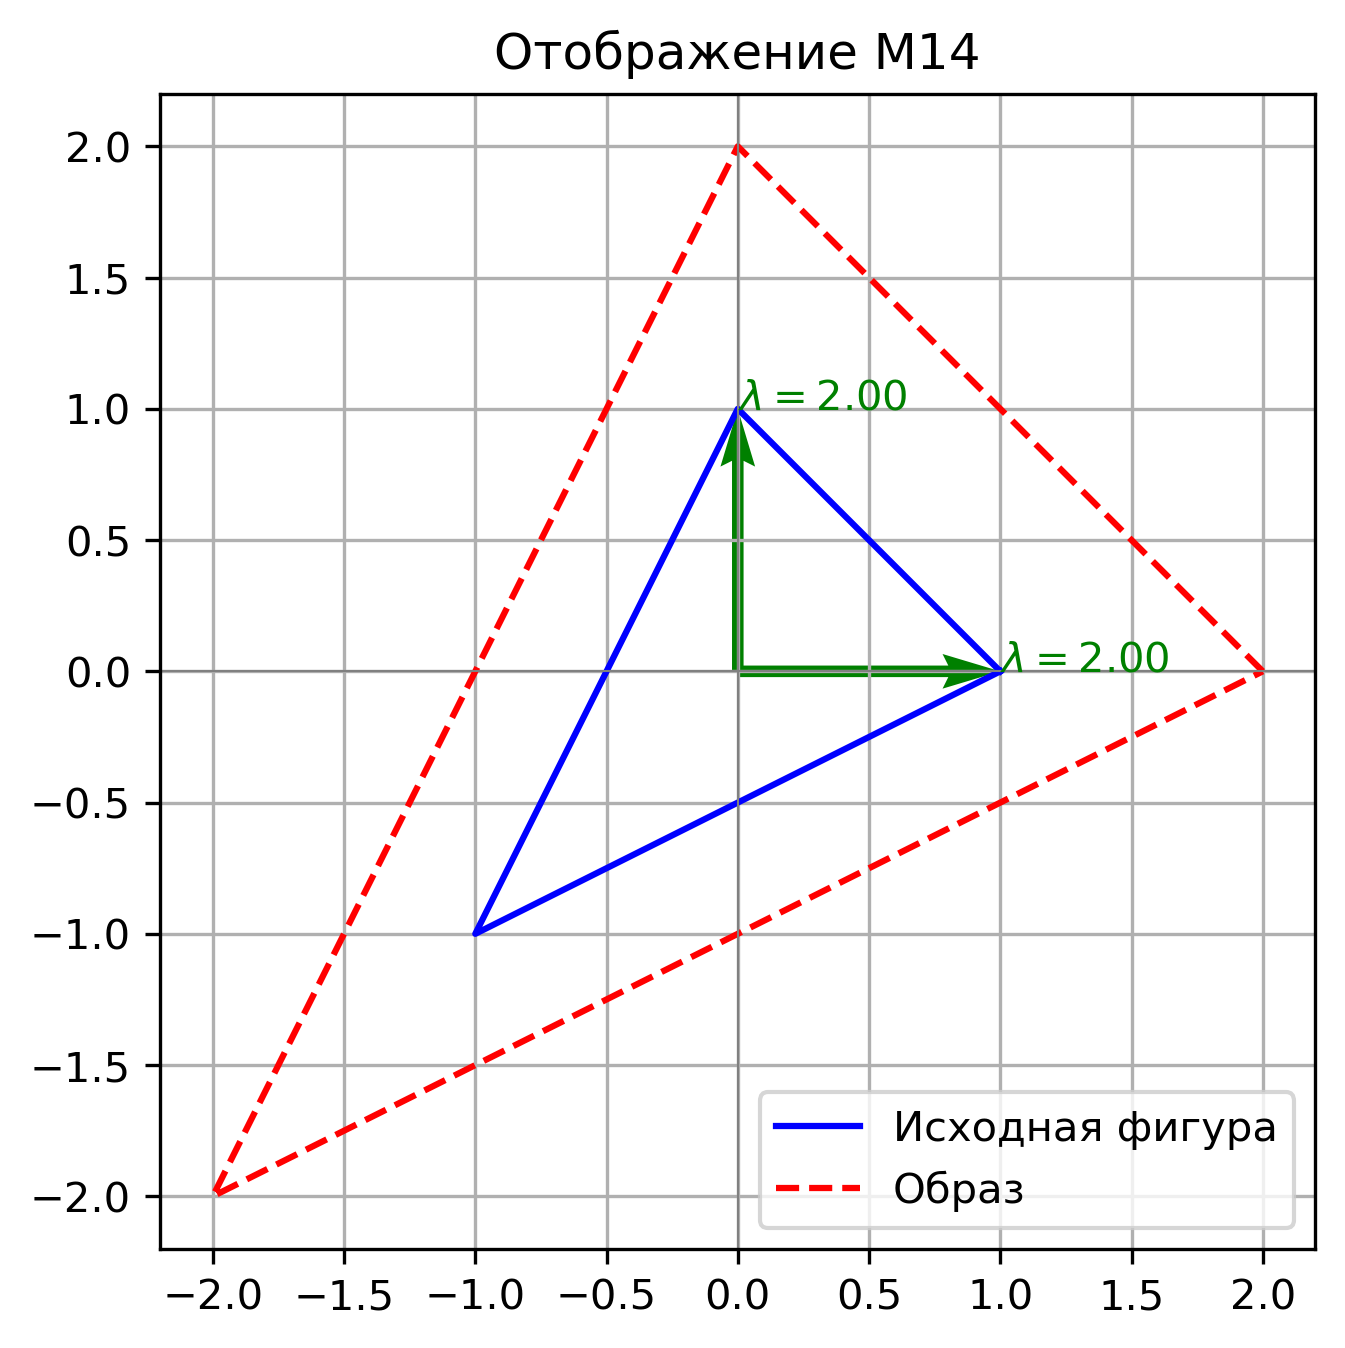
\includegraphics[width=\linewidth]{plots/M14.png}
    \caption{$M_{14}$}
  \end{subfigure}\hfill
  \begin{subfigure}[b]{0.3\textwidth}
    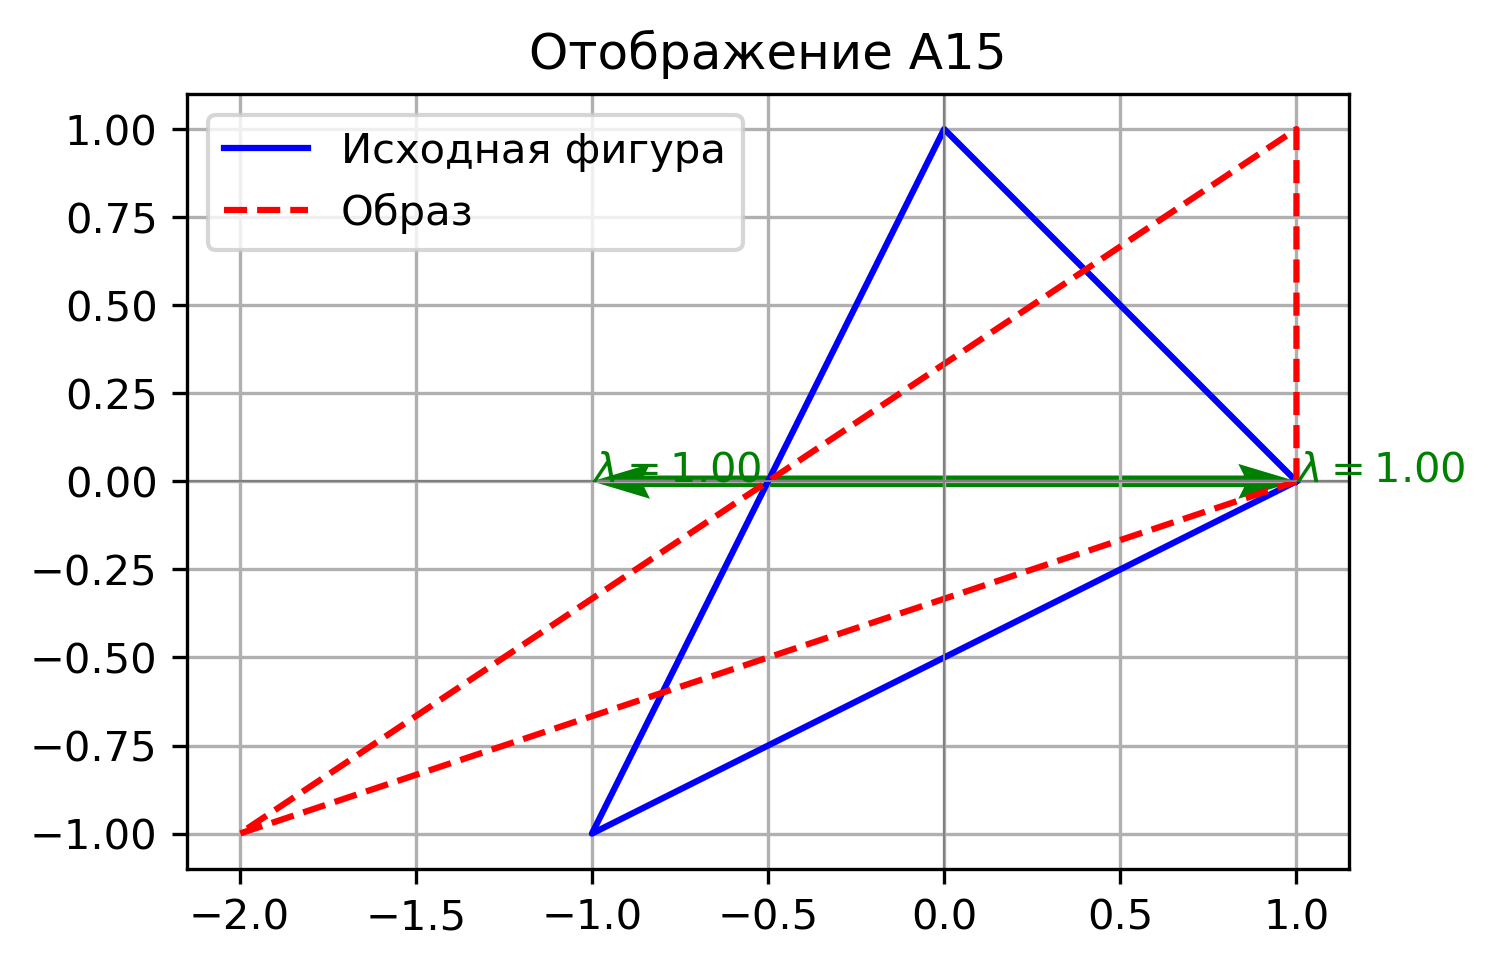
\includegraphics[width=\linewidth]{plots/A15.png}
    \caption{$A_{15}$}
  \end{subfigure}

  \vspace{0.5cm}

  \begin{subfigure}[b]{0.3\textwidth}
    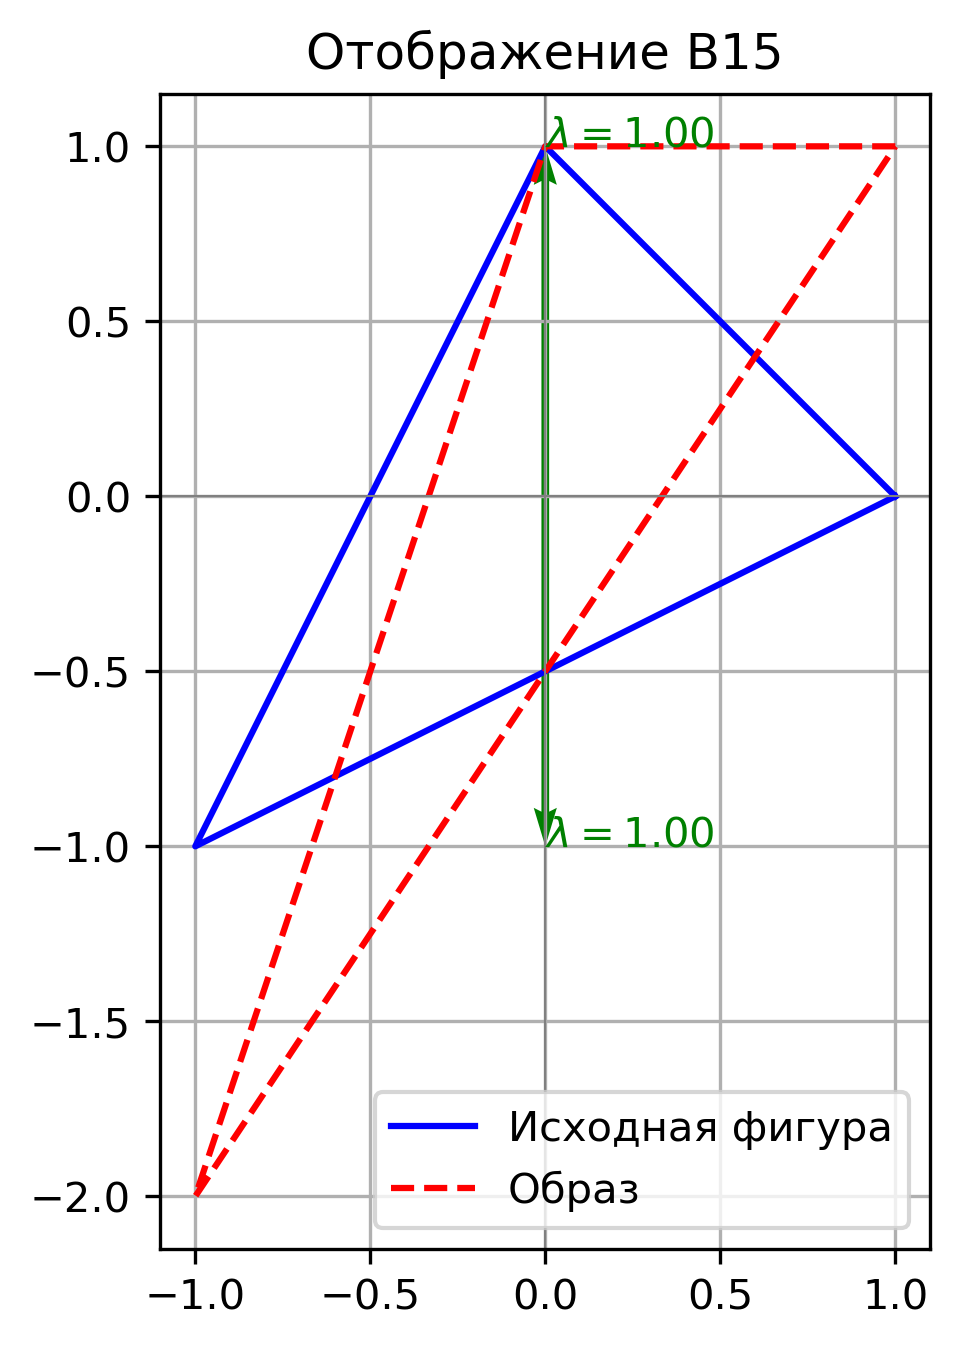
\includegraphics[width=\linewidth]{plots/B15.png}
    \caption{$B_{15}$}
  \end{subfigure}\hfill
  \begin{subfigure}[b]{0.3\textwidth}
    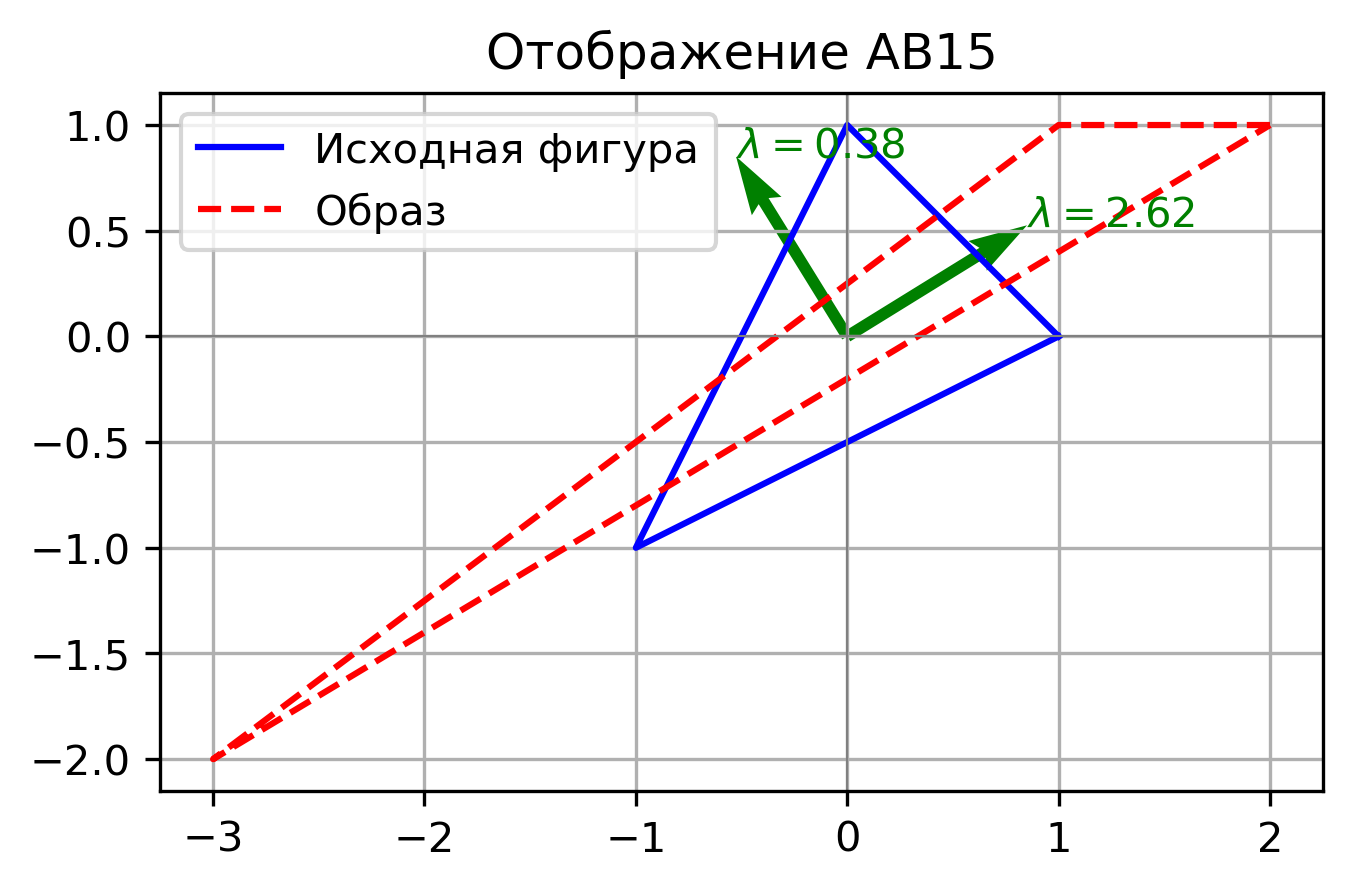
\includegraphics[width=\linewidth]{plots/AB15.png}
    \caption{$A_{15}B_{15}$}
  \end{subfigure}\hfill
  \begin{subfigure}[b]{0.3\textwidth}
    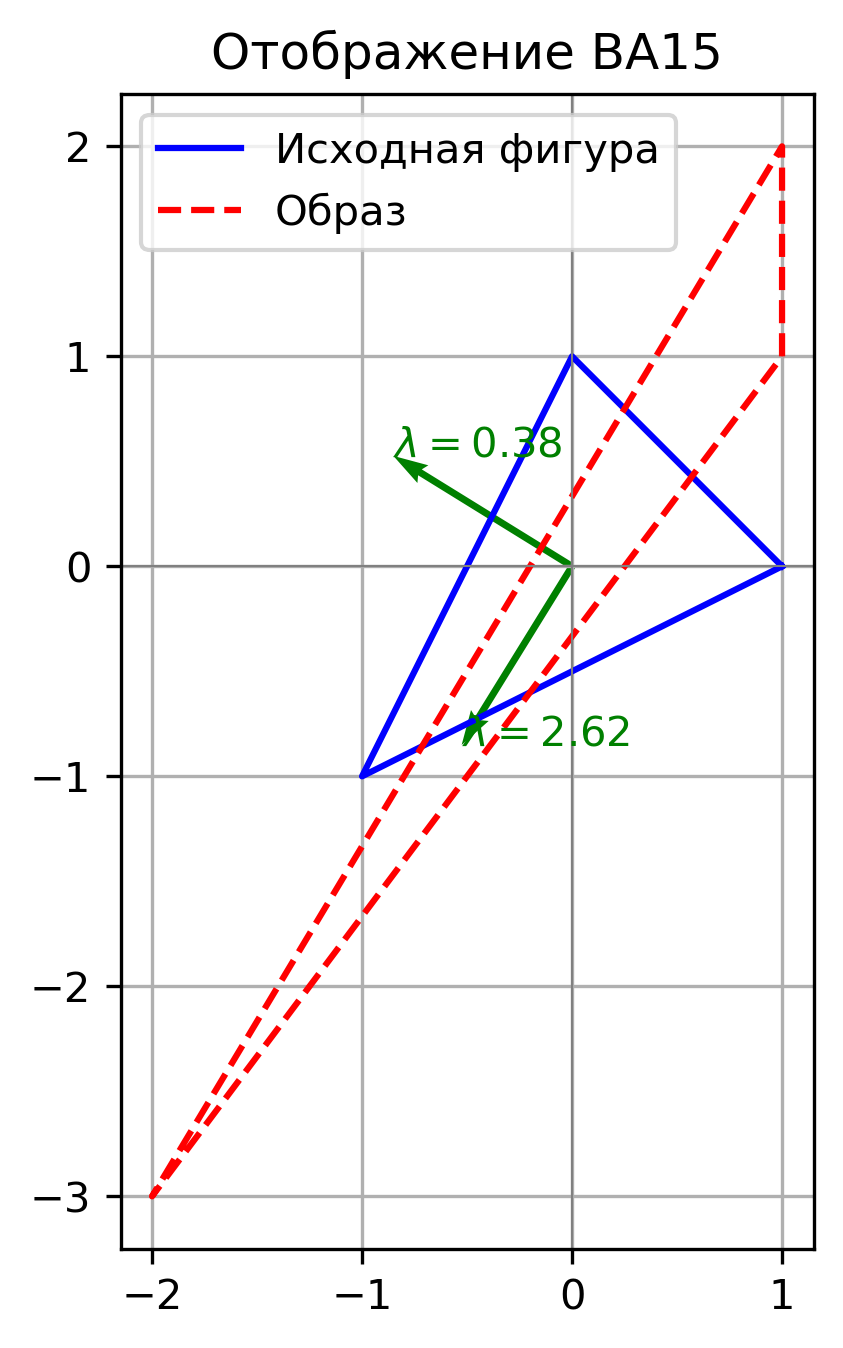
\includegraphics[width=\linewidth]{plots/BA15.png}
    \caption{$B_{15}A_{15}$}
  \end{subfigure}
  \caption{Отображения $M_{13}$–$BA_{15}$}
\end{figure}

\clearpage

\begin{figure}[H]
  \centering
  \begin{subfigure}[b]{0.3\textwidth}
    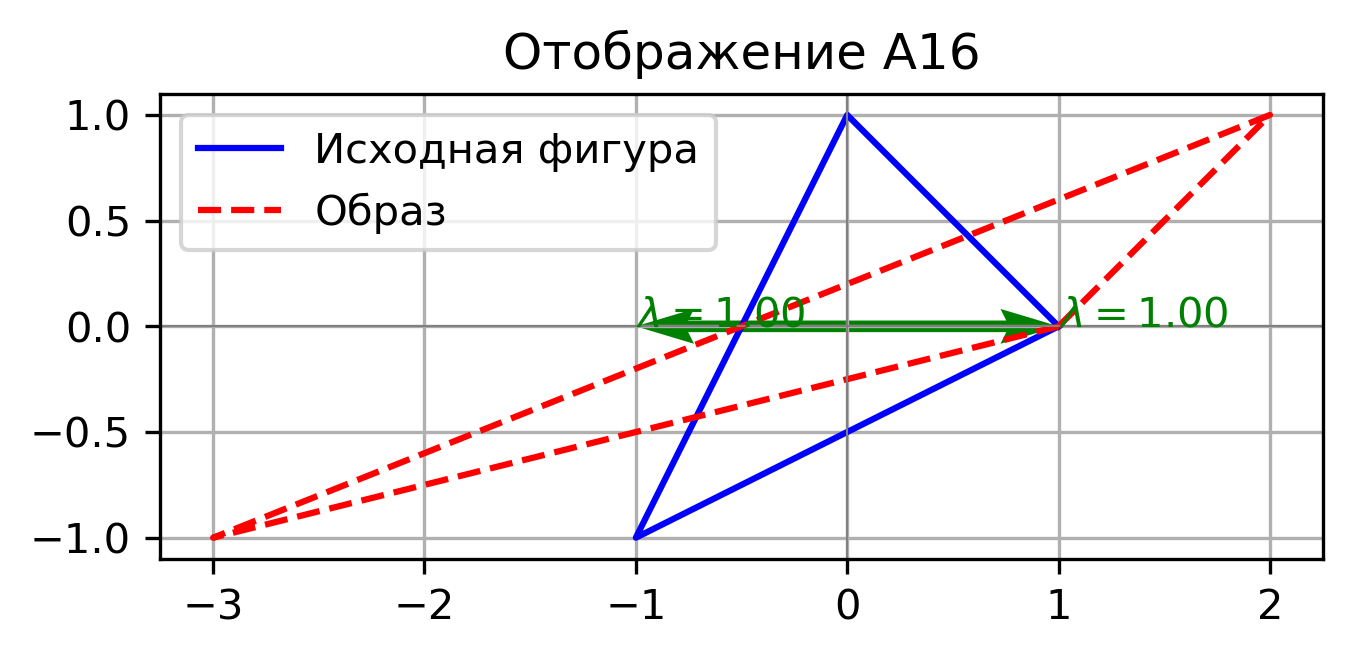
\includegraphics[width=\linewidth]{plots/A16.png}
    \caption{$A_{16}$}
  \end{subfigure}\hfill
  \begin{subfigure}[b]{0.3\textwidth}
    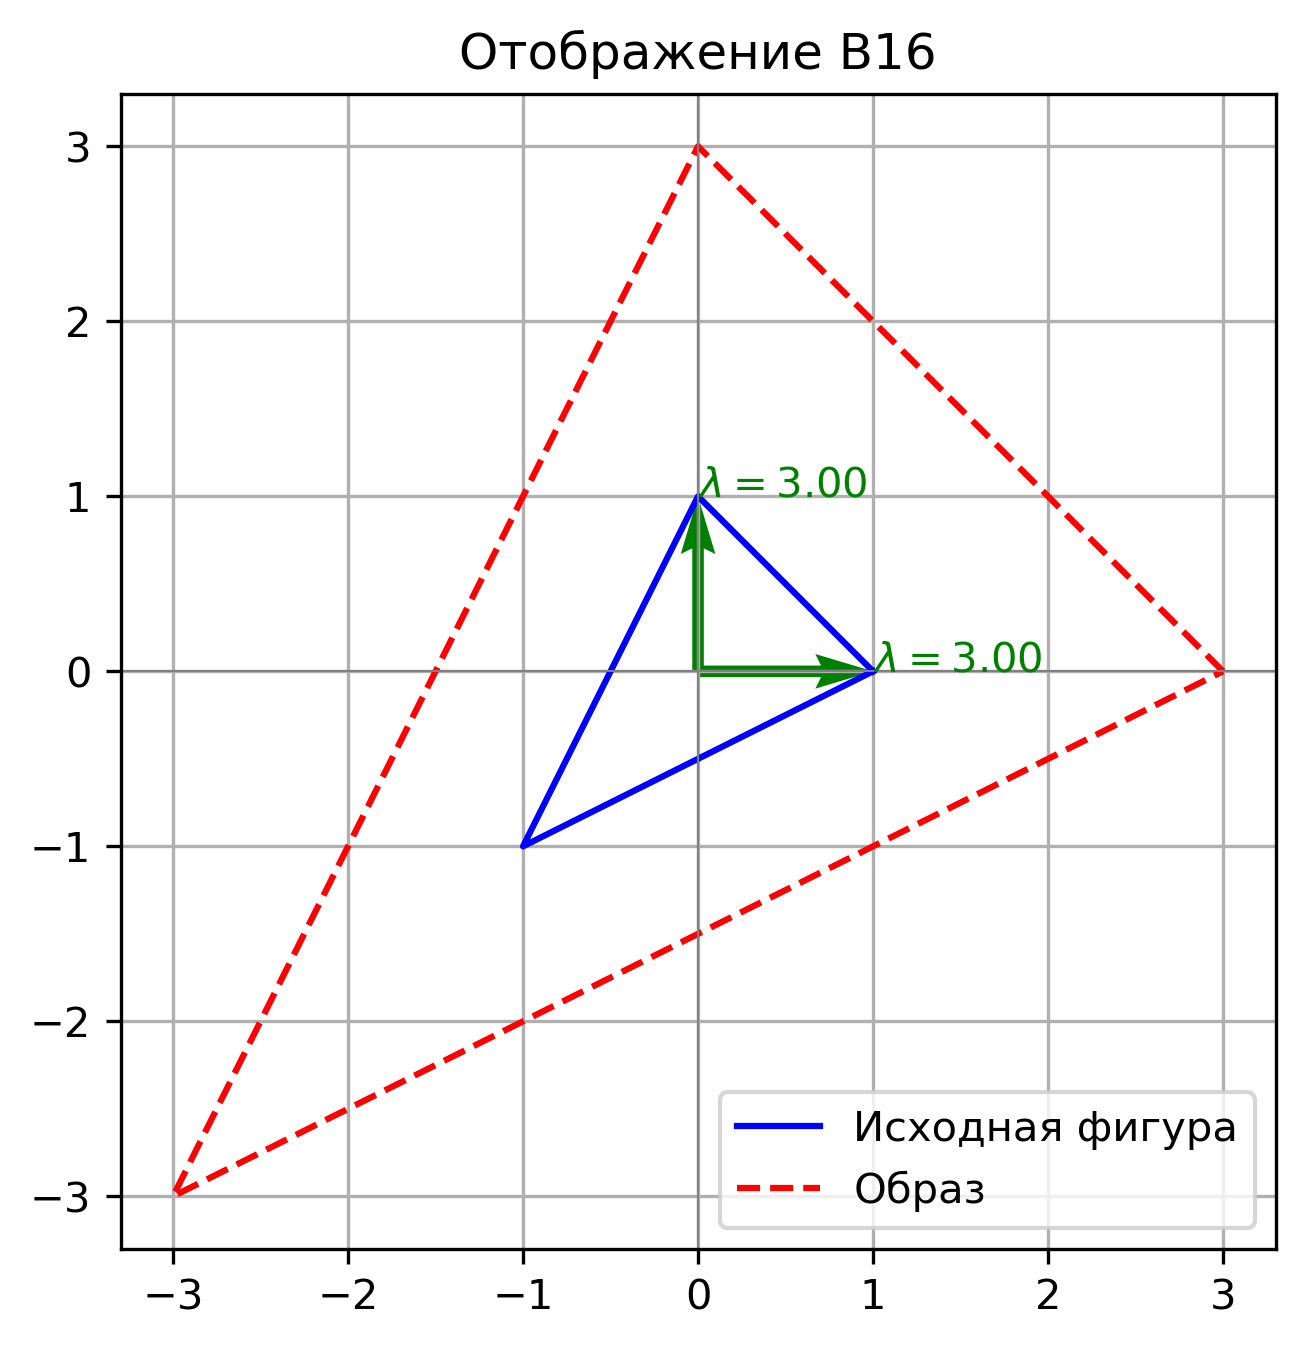
\includegraphics[width=\linewidth]{plots/B16.png}
    \caption{$B_{16}$}
  \end{subfigure}\hfill
  \begin{subfigure}[b]{0.3\textwidth}
    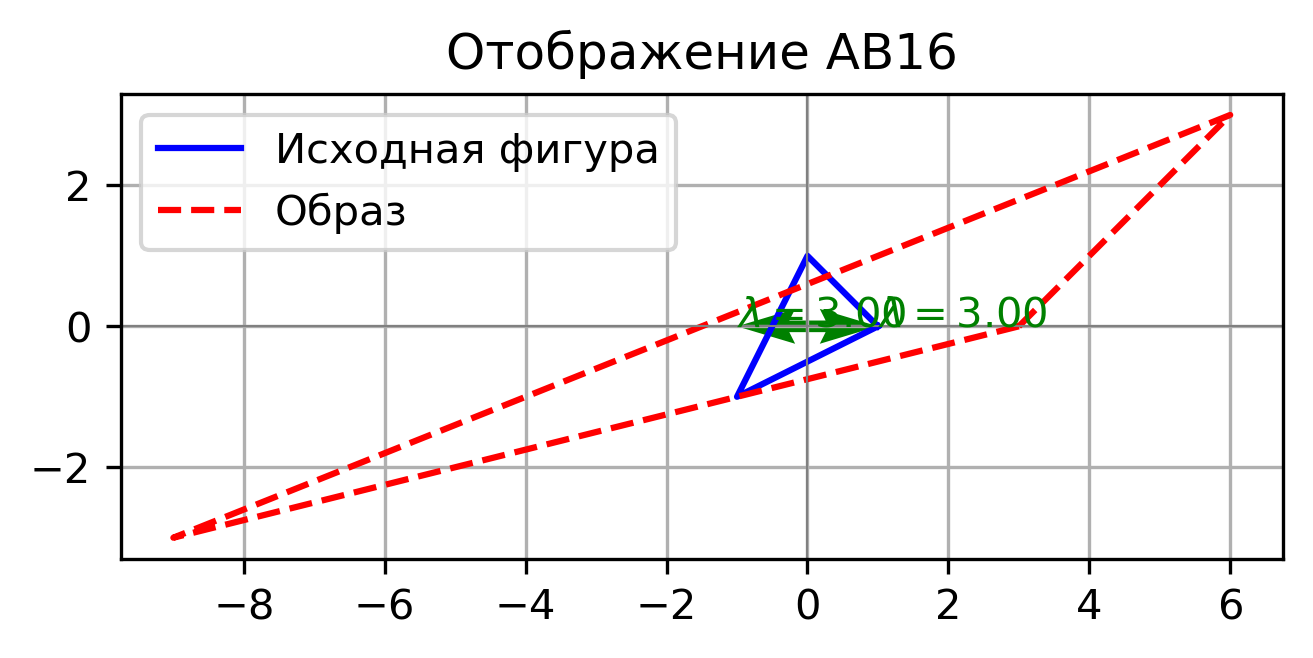
\includegraphics[width=\linewidth]{plots/AB16.png}
    \caption{$A_{16}B_{16}$}
  \end{subfigure}

  \vspace{0.5cm}

  \begin{subfigure}[b]{0.3\textwidth}
    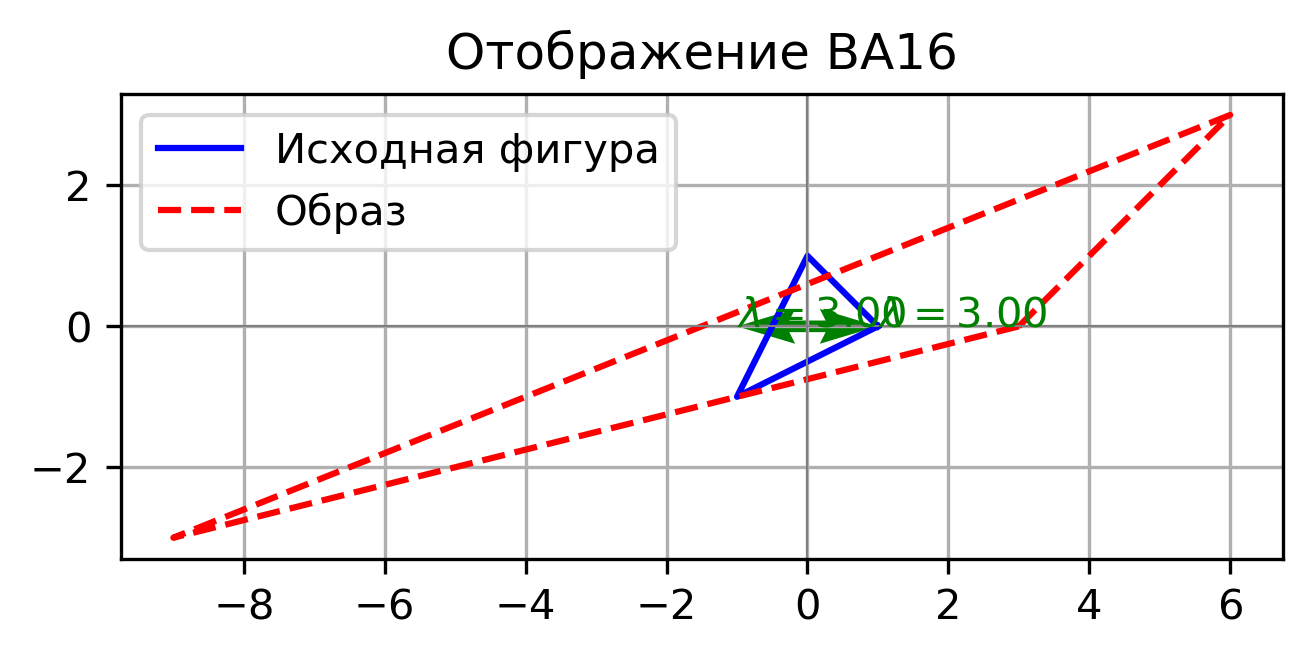
\includegraphics[width=\linewidth]{plots/BA16.png}
    \caption{$B_{16}A_{16}$}
  \end{subfigure}
  \caption{Отображения $A_{16}$–$BA_{16}$}
\end{figure}

\clearpage
\end{document}